\documentclass[useAMS,usenatbib,referee]{bio}
%\documentclass[12pt]{article}
%\usepackage{fullpage}
\usepackage{url,color}
\usepackage{rotating,epsfig}
\usepackage{verbatim}
\usepackage{amsmath,amsfonts,amssymb,amsthm}
\usepackage{natbib}
\usepackage{lscape}
\usepackage{textcomp}
\usepackage[ruled,vlined]{algorithm2e}
\usepackage{graphicx}
\usepackage{multirow}

%\renewcommand{\baselinestretch}{1.5}

\def\dfrac#1#2{\displaystyle{{#1}\over{#2}}}
\def\dsum#1#2{\displaystyle\sum_{#1}^{#2}}
%\newtheorem{theorem}{Theorem}
\newcommand{\RR}{{\rm I\! R}}
\newcommand{\eg}{{e.g.}}
\newcommand{\ie}{{i.e.}}
\newcommand{\argmin}{\operatornamewithlimits{argmin}}
\newcommand{\bs}{\boldsymbol}
\newcommand{\eps}{\epsilon}
%\newcommand*\samethanks[1][\value{footnote}]{\footnotemark[#1]}

\newcommand*{\Cdot}[1][1.25]{%
  \mathpalette{\CdotAux{#1}}\cdot%
}
\newdimen\CdotAxis
\newcommand*{\CdotAux}[3]{%
  {%
    \settoheight\CdotAxis{$#2\vcenter{}$}%
    \sbox0{%
      \raisebox\CdotAxis{%
        \scalebox{#1}{%
          \raisebox{-\CdotAxis}{%
            $\mathsurround=0pt #2#3$%
          }%
        }%
      }%
    }%
    % Remove depth that arises from scaling.
    \dp0=0pt %
    % Decrease scaled height.
    \sbox2{$#2\bullet$}%
    \ifdim\ht2<\ht0 %
      \ht0=\ht2 %
    \fi
    % Use the same width as the original \cdot.
    \sbox2{$\mathsurround=0pt #2#3$}%
    \hbox to \wd2{\hss\usebox{0}\hss}%
  }%
}

\newcommand*{\test}[1]{%
  \text{%
    \setlength{\fboxsep}{0pt}%
    \setlength{\fboxrule}{.1pt}%
    \fbox{$#1$}%
  }%
}

\begin{document}

\title{Penalized Regression Method to Find Abnormality in brain network of Alzheimer's Disease}

% List of authors, with corresponding author marked by asterisk
\author{DONGHYEON YU\\[2pt] 
\textit{Department of Statistics, Keimyung University, Daegu, South Korea}
\\[2pt]
SANG HAN LEE$^{\ast}$\\ [2pt]
\textit{ 
Center for Biomedical Imaging and Neuromodulation, Nathan Kline Institute for Psychiatric Research, Orangeburg, NY 10962, USA}
\\[2pt]
{shlee@nki.rfmh.org}\\[2pt]
JOHAN LIM \\[2pt]
\textit{Department of Statistics, Seoul National University, Seoul, South Korea} \\[2pt]
GUANGHUA XIAO\\[2pt]
\textit{ 
University of Texas Southwestern Medical Center, Dallas, TX 75390, USA}
\\[2pt]
R. CAMERON CRADDOCK\\ [2pt]
\textit{ 
Center for Biomedical Imaging and Neuromodulation, Nathan Kline Institute for Psychiatric Research, Orangeburg, NY 10962, USA}
\\[2pt]
BHARAT B. BISWAL  \\[2pt]
\textit{ 
Department of Biomedical Engineering, New Jersey Institute of Technology, Newark, NJ 07102, USA
}
\\[2pt]
}

% Running headers of paper:
\markboth%
% First field is the short list of authors
{D. Yu and others}
% Second field is the short title of the paper
{Penalized Regression Method for differential network}

\maketitle

% Add a footnote for the corresponding author if one has been
% identified in the author list
\footnotetext{To whom correspondence should be addressed.}


\begin{abstract}
{In this paper, we propose a procedure to find differential networks in partial correlations from high-dimensional multivariate data. We estimate the precision matrices and their differences by solving a penalized regression-based least square problem. We assume sparse differences between two precision matrices, not matrices themselves. Thus, we impose $\ell_2$ penalty on
partial correlations from elements of precision matrices while $\ell_1$ penalty on their differences. We apply the proposed procedure to finding differential functional connectivity in the resting brain between normal and Alzheimer's disease patients.}
{ Precision matrix; fMRI; functional connectivity; Gaussian graphical model; $\ell_1$ penalty; penalized least squares.}
\end{abstract}


%\baselineskip24pt
\section{Introduction}

\iffalse
At the macroscopic scale, the human connectome is an undirected weighted graph that represents connectivity between every pair of anatomically distinct areas in the brain\cite{Craddock2013Connectomes}. For functional connectomes, brain areas correspond to functionally homogeneous patches of cortex and edges correspond to functional connectivity between nodes, which is inferred from temporal correlations between time series of activity measured at the corresponding brain areas\cite{Craddock2013Connectomes,Varoquaux2013}. Functional connectivity can be estimated using data from a variety of different imaging modalities and experimental conditions, but resting state functional magnetic resonance imaging (rsfMRI) data is popularly used given its noninvasiveness, high spatial resolution, and general applicability across individuals regardless of age, brain state, or disability\cite{Biswal1995}. When estimated in these ways, human connectome graphs have been shown to be reproducible across time\cite{shehzad2009} and individuals\cite{damasoix}, which is driving considerable optimism that they can provide stable markers of inter-individual variability in phenotype (e.g., disease states, disease severity, IQ, personality, etc). Mapping phenotypes to connectome graphs is a challenging problem that is commonly reduced to estimating a graph per individual using bivariate Pearson's correlations and submitting the results to edge-wise univariate statistical tests \cite{craddock2013connectome, varoquaux2013}. This methodology is problematic for two reasons: bivariate Pearson's correlation cannot distinguish the shared variance between two areas from their common variance with other brain areas and it results in a very large number of comparisons that serve to reduce detection power. 

Partial correlation is an attractive alternative to Pearson's correlation for estimating functional connectome graphs, since it is not prone to artefactual correlations arising from shared variance with brain areas other than those being compared\cite{Varoquaux2013}. Although the entire partial correlation matrix can be obtained by from the inverse of the covariance matrix (precision matrix), rsfMRI data tends to contain many more brain areas than independent observations ($p >> n$), resulting in an ill-posed problem. This problem has been addressed in the neuroimaging literature by using regularized estimators of the precision matrix, such as Graphical LASSO \citep{Meinshausen:2006,Yuan:2007,Rothman:2008}, that enforce sparsity to find a unique solution.  


1. Can use partial correlation to estimate each individual's connectome separately, and submit results to group level analysis. Separately estimating the precision matrix for each subject, it is not quite clear how the group level precision matrix should be estimated - the mean of the subject level matrices may not be the best thing.  - these estimates are noisy, and could be improved by sharing information across individuals

2. Can estimate individual level precisions with a group regularization, enforces the same sparsity structure for each individual. This method enforces a high level of sparsity which may not be ecologically valid, because brain networks maybe more dense than this method assumes. -- requires an assumption of level of sparsity and normality

3. Rather than focusing on the estimation of precision matrices for each individual or each group, we propose to directly estimate the differences between groups. This enables us to relax the sparsity requirement for each group precision matrix, and instead impose this sparsity constraint on the between-group differences. Sparsity of the differences will improve the interpretability of the results.



since it distinguishes 

measures the linear dependency between two brain areas independent of commmon variance from all other areas of the brain. 
\fi


At the macroscopic scale, the human connectome is an undirected weighted graph that represents connectivity between every pair of anatomically distinct areas in the brain \citep{Craddock2013Connectomes}. For functional connectomes, brain areas correspond to functionally homogeneous patches of cortex and edges correspond to functional connectivity between nodes, which is inferred from temporal correlations between time series of activity measured at the corresponding brain areas \citep{Craddock2013Connectomes,Varoquaux2013}. 

Functional connectivity can be estimated using data from a variety of different imaging modalities and experimental conditions, but resting state functional magnetic resonance imaging (rsfMRI) data is popularly used given its noninvasiveness, high spatial resolution, and general applicability across individuals regardless of age, brain state, or disability. When estimated in these ways, human connectome graphs have been shown to be reproducible across time \citep{shehzad2009} and individuals \citep{damasoix}, which is driving considerable optimism that they can provide stable markers of inter-individual variability in phenotype (e.g., disease states, disease severity, IQ, personality, etc). 
Thus, this study is motivated by a rsfMRI study of Alzheimer's disease (AD). Researchers are interested to find whether and where there is any abnormality in brain function of patients with AD based on rsfMRI. In other words, people are interested to estimate intrinsic functional connectivity in brain and/or their differences between different populations, e.g., healthy control (HC) versus patients with AD.

Mapping phenotypes to connectome graphs is a challenging problem that is commonly reduced to estimating a graph per individual using bivariate Pearson's correlations and submitting the results to edge-wise univariate statistical tests. This methodology is problematic for two reasons: bivariate Pearson's correlation cannot distinguish the shared variance between two areas from their common variance with other brain areas and it results in a very large number of comparisons that serve to reduce detection power. 
Partial correlation is an attractive alternative to Pearson's correlation for estimating functional connectome graphs, since it is not prone to artefactual correlations arising from shared variance with brain areas other than those being compared. 
In addition, a population-level inference on graphs is needed in comparing them.

Statistically, the problem of finding abnormality in AD based on rsfMRI can be viewed as estimating two partial correlation graphs and their differences. 
Although the entire partial correlation matrix can be obtained from the inverse of the covariance matrix (precision matrix), rsfMRI data tends to contain many more brain areas than independent observations ($p >> n$), resulting in an ill-posed problem. 

In recent literature, a number of methods have been proposed to estimate the precision matrix for high-dimensional data. Many of proposed methods are based on Gaussian graphical model \citep{Meinshausen:2006,Yuan:2007,Rothman:2008}, that enforce sparsity to find a unique solution. 
Later, \citet{Danaher:2014} proposed the joint graphical lasso (JGL) method, which has some advantages over the approach of separate estimates in the flexibility to control both the sparsity of precision matrices and their similarity.
In detail, assume that data of size $n_i$ are from $N \big(0, \Sigma_i\big)$ for the $i$-th population, $i=1,2,\ldots, I$.
Let $S_i$ be the sample covariance matrix of the $i$-th population and $\Omega_i\equiv \Sigma_i^{-1}$ be the precision matrix of the $i$-th population.
JGL method maximizes
\begin{eqnarray*}
l(\Omega_1,\ldots,\Omega_I)
&=& \sum_{i=1}^I n_i \Big\{ \log\det
\Omega_i - {\rm tr}(\Omega_i {S}_i ) \Big\}  - \mathcal{P} \big( \Omega_1,\ldots,\Omega_I \big),
\end{eqnarray*}
where $\det \Omega_i$ denotes the determinant of $\Omega_i$, ${\rm tr}(A)$ is the trace of $A$, and $\mathcal{P} \big( \Omega_1,\ldots,\Omega_I \big)$ is a given penalty function. JGL method considers two useful penalties, the fused lasso penalty to find differences in precision matrices and the group lasso penalty to find a common non-sparse structure.
However, these graphical models enforces a high level of sparsity which may not be ecologically valid, because brain networks may be more dense than this method assumes \citep{Ryali2012}.

Alternative approach would be to directly estimate the differences.  \citet{Zhao:2014} proposed to directly estimate the differences between two precision matrices as the solution to
\begin{equation} \label{eqn:direct} 
\mbox{minimize }  \big\| \Delta\big\|_1 \quad 
\mbox{subject to} ~~ \big\| {\bf S}_1 \Delta {\bf S}_2 -  {\bf S}_1 + {\bf S}_2 \big\|_{\infty} \le \lambda,
\end{equation} 
where $\Delta = \Omega_2-\Omega_1$ and $\lambda$ is a non-negative tuning parameter. 
To solve (\ref{eqn:direct}), they rewrite the problem as the well-known regression problem named as the Dantizg selector by \citet{Candes:2005}.
An obvious advantage of this over the graphical model is that it does not require to estimate the precision matrices. Hence, the sparsity on the precision matrices is not required, which allows networks to have hubs. It also dose not require the normality. However, their method demands costly memory and time as stated in their study. This might not be practical in rsfMRI study since both $p$ and $n$ can be large.

In this paper we propose a computationally efficient method to find abnormality in the brain functional connectivity of patients with AD for high-dimensional rsfMRI study.
Rather than focusing on the estimation of precision matrices for each individual or each group, we propose to directly estimate the differences between groups as in \citet{Zhao:2014}. This enables us to relax the sparsity requirement for each group precision matrix, and instead impose the sparsity constraint on the between-group differences. Sparsity of the differences will improve the interpretability of the results.

Our work here exploits the penalized regression approach, which is computationally efficient comparing to \citet{Zhao:2014}. The penalized regression solves a least square problem to estimate sparse precision matrix $\Omega=\big(\omega_{kl} \big)_{1\le k,l\le p}$. 
In detail, suppose ${\bf X}= (X_1 ,\cdots, X_p)^T$ is a random vector of mean $0$ and a positive definite covariance matrix $\Sigma$.  
Denote the partial correlation between $x_i$ and $x_j$ by $\rho_{ij}$.
It is known that, for every $k=1,2,\ldots,p$,
\begin{equation} \label{eqn:pcorr_reg}
X_k = \sum_{l \neq k} \beta_{kl} X_l + \epsilon_k,
\end{equation}
where $\beta_{kl}=- \omega_{kl}/\omega_{kk} = \rho_{kl} \sqrt{ \omega_{ll} / \omega_{kk} }$, $\rho_{kl}=-\omega_{kl}/\sqrt{\omega_{kk}\omega_{ll}}$ and $\epsilon_k$ is uncorrelated with $X_{-k}=\{ X_l~|~ l \neq k,~
l=1,2,\ldots,p\}$ and has variance $1/\omega_{kk}$. 
Motivated by identity ({\ref{eqn:pcorr_reg}), \citet{Meinshausen:2006} proposed a penalized regression approach of solving a set of $p$ regression problems with $\ell_1$-regularization, that is, for $k=1,2,\ldots,p$,
\begin{eqnarray*} \label{eqn:regress_mb}
\mbox{minimize} ~~ \sum_{j=1}^n \big( x_{jk} - \sum_{l\neq k}
\beta_{kl} x_{jl}\big)^2  + \lambda \sum_{l \neq k} |\beta_{kl}|,
\end{eqnarray*}
where ${\bf x}_j=\big(x_{j1},x_{j2},\ldots,x_{jp}\big)^T$ for $j=1,\ldots,n$, are independent and identically distributed (IID) copies of ${\rm X}$.
Later, \citet{Peng:2009} proposed the sparse partial correlation estimation (SPACE) method which minimizes the weighted sum of $p$ objectives:
\begin{equation} \label{eqn:peng}
\sum_{k=1}^p w_k \left\{ \sum_{j=1}^n \big( x_{jk} - \sum_{l\neq k}
\beta_{kl}
     x_{jl}\big)^2 \right\} + \lambda \sum_{k=1}^p\sum_{l \neq k} |\rho_{kl}|,
\end{equation}
where $w_k$s are non-negative weights. 
SPACE method has a couple of advantages over the method by \citet{Meinshausen:2006} in estimating the precision matrix and the graph structure. It allows the graph to have hubs and also provides a symmetric precision matrix by minimizing weighted sum of $p$ least squares. 
More importantly, when weights $w_k= \omega^2_{kk}$ and imposing penalty on $\omega_{kl}$, the weighted sum of ({\ref{eqn:peng}) becomes convex and allows an algorithm to find the global optimum \citep{Khare2014}. 
Hence, we extend SPACE to our differential network problem, i.e., estimating two partial correlation graphs and their differences.

Suppose ${\bf X}^{(i)} =\big(X^{(i)}_{1},X^{(i)}_{2},\ldots,X^{(i)}_{p}\big)$ for $i=1,2$ is 
a random vector from the $i$-th population (e.g., $i=1$ for the normal population and $i=2$ for the population of the patients with AD). 
Assume that ${\bf X}^{(i)} \sim (0,\Sigma_i)$ and the precision matrix $\Omega_i=\big(\omega_{kl}^{(i)} \big)_{1\le k,l\le p}$. 
Then, for every
$k=1,2,\ldots,p$,
\begin{eqnarray} 
X^{(1)}_{k} &=& \sum_{l \neq k} \beta^{(1)}_{kl} X^{(1)}_{l} + \epsilon^{(1)}_{k} = \sum_{l \neq k} \rho^{(1)}_{kl} \tilde{X}^{(1)}_{l(k)} + \epsilon^{(1)}_{k}, \label{eqn:iden} \nonumber\\
X^{(2)}_{k} &=& \sum_{l \neq k} \beta^{(2)}_{kl} X^{(2)}_{l} + \epsilon^{(2)}_{k} =\sum_{l \neq k} \rho^{(2)}_{kl} \tilde{X}^{(2)}_{l(k)} + \epsilon^{(2)}_{k}, \nonumber
\end{eqnarray}
where $\tilde{X}^{(i)}_{l(k)}= \sqrt{\frac{\omega^{(i)}_{ll}}{\omega^{(i)}_{kk}} } X^{(i)}_{l}$. 
In this paper, we propose to minimize a penalized regression function:
\begin{equation} \label{eqn:main}
\begin{array}{lll}  \medskip
&& \displaystyle
 \sum_{k=1}^p \bigg\{w^{(1)}_{k} \sum_{j=1}^{n_1} \big(X_{jk}^{(1)} -  \sum_{l \neq k} \rho^{(1)}_{kl} \tilde{X}_{jl(k)}^{(2)} \big)^2 + w^{(2)}_{k}
\sum_{j=1}^{n_2} \big( X_{jk}^{(2)} - \sum_{l \neq k} \rho^{(2)}_{kl} \tilde{X}_{jl(k)}^{(2)}  \big)^2 \bigg\}  \\
&& \displaystyle \qquad \qquad
+ \lambda_1 \mathcal{P}_1\big( \bs{\rho^{(1)}},\bs{\rho^{(2)}} \big) + \lambda_2 \mathcal{P}_2 \big( \bs{\rho^{(2)}} - \bs{\rho^{(1)}} \big),
\end{array}
\end{equation}
where ${\bf X}^{(i)}_j=\big(X_{j1}^{(i)}, X_{j2}^{(i)},\ldots,X_{jp}^{(i)}\big)$ are IID copies
of ${\bf X}^{(i)}$ for $j=1,2,\ldots,n_i$, $w^{(i)}_{k}$s are nonnegative weights, $\lambda_i$s are non-negative tuning parameters, $ \mathcal{P}_1(\cdot) ,
\mathcal{P}_2(\cdot) $ are penalty functions and $\bs{\rho^{(i)}}=(\rho^{(i)}_{12},\ldots,\rho^{(i)}_{(p-1)p})^T$. 


The paper is organized as follows. In Section 2, we describe the proposed model and the algorithm to solve the penalized regression problem that we consider. We also discuss the selection of tuning parameters. In Section 3, we numerically investigate the performance of the proposed procedure along with the comparison to other methods. In Section 4, we apply our proposal to a resting-state fMRI study for AD. In this example, we find the differences in functional connectivity in resting brain between healthy control and patients with AD. In Section 5, we conclude the paper with a brief discussion.


\section{Method}


\subsection{Model}
The $p$-variate vector of observations on the $j$-th subject in the $i$-th network is denoted by $\mathbf{Y}^{(i)}_j = (Y_{j1}^{(i)}, \ldots, Y_{jp}^{(i)})^{\rm
T}$, $j=1, \ldots, n_i$, and $i=1,2$.
When random samples $\mathbf{Y}^{(i)}_1, \dots, \mathbf{Y}^{(i)}_{n_i}$ from
the $i$-th network follow the $p$-variate distribution 
$(\bs{\mu}_i,\bs{\Sigma}_i)$ with $\bs{\Omega}_i=
\big( \omega^{(i)}_{kl} \big)_{1 \le k,l \le p}$,
we can transform $\mathbf{Y}^{(i)}_{j}$ into $\tilde{\mathbf{Y}}^{(i)}_j = \mathbf{Y}^{(i)}_j - \frac{1}{n_i} \sum_{j=1}^{n_i} \mathbf{Y}^{(i)}_j$,
which approximately follows $(\mathbf{0},\bs{\Sigma}_i)$ for $j=1,\ldots,n_i$ and $i=1,2$.
Hence, without loss of generality, we assume that $\mathbf{Y}^{(i)}_j$ follows distribution $(\mathbf{0},\bs{\Sigma}_i)$ for $j=1,\ldots,n_i,~i=1,2$.

In order to formulate the problem in a linear model as \citet{Peng:2009}, we let
$\mathbf{Y}^{(i)}_{\bullet k} = \big(Y_{1k}^{(i)}, Y_{2k}^{(i)},\ldots,Y_{n_ik}^{(i)} \big)^T$ as the column vector for $n_i$ observations of the $k$-th variate.
Then, we concatenate all observations of $p$ variates into a vector,  
$\mathbf{Y} = \big(
 {\mathbf{Y}^{(1)}_{\bullet 1}}^T, \ldots,{\mathbf{Y}^{(1)}_{\bullet p}}^T;
 {\mathbf{Y}^{(2)}_{\bullet 1}}^T, \ldots, {\mathbf{Y}^{(2)}_{\bullet p}}^T \big)^T$. 
Likewise, diagonal elements of two precision matrices are vectorized as
$\bs{\omega}_D=\big(\bs{\omega}_{D_1}^T, \bs{\omega}_{D_2}^T\big)^T =
(\omega^{(1)}_{11},\ldots,\omega^{(1)}_{pp};\omega^{(2)}_{11},\ldots,\omega^{(2)}_{pp})^T.$

Finally, we let 
$
\mathcal{X}^{(i)}_{k,l}
= \big( \mathbf{0}_{n_i(k-1)\times 1}^{T},
{\mathbf{Y}^{(i)}_{\bullet l(k)}}^T, \mathbf{0}_{n_i(l-k-1)\times 1}^T
, {\mathbf{Y}^{(i)}_{\bullet k(l)}}^T, \mathbf{0}_{n_i(p-l)\times 1}^T
\big)^T
$ where
$\mathbf{Y}^{(i)}_{\bullet k(l)} = \sqrt{\frac{\omega^{(i)}_{kk}}{\omega^{(i)}_{ll}}}
\mathbf{Y}^{(i)}_{\bullet k}$, and
\begin{equation*} \label{xmat}
\mathcal{X}=
\begin{pmatrix}
\begin{array}{cc}
{\mathcal{X} }^{(1)} & {\bf 0}\\
{\bf 0} & {\mathcal{X}}^{(2)}
\end{array}
\end{pmatrix}
=
\begin{pmatrix}
\begin{array}{cccccccc}
 \mathcal{X}_{1,2}^{(1)}&  \mathcal{X}_{1,3}^{(1)}&
 \cdots& \mathcal{X}^{(1)}_{(p-1),p}& {\bf 0}& {\bf 0}&
 \cdots&
 {\bf 0} \\
{\bf 0}&  {\bf 0}&
 \cdots& 0 &\mathcal{X}_{1,2}^{(2)}&  \mathcal{X}_{1,3}^{(2)}&
  \cdots& \mathcal{X}^{(2)}_{(p-1),p}
 \end{array}
 \end{pmatrix}.
\end{equation*}

Then, the random  vector $\mathbf{Y}$ and the matrix $\mathcal{X}$ satisfy a linear model
\begin{equation*} \label{eqn:linear}
\mathbf{Y}= \mathcal{X} \bs{\rho} + \bs{\epsilon,}
\end{equation*}
where
\begin{equation} \nonumber
\bs{\epsilon} =
\begin{pmatrix}
\begin{array}{cccccc}
\bs{\epsilon}_{1,1}^{ T},& \cdots ,&\bs{\epsilon}_{1,p}^{ T}, &
\bs{\epsilon}_{2,1}^{ T} ,& \cdots ,& \bs{\epsilon}_{2,p}^{ T}
\end{array}
\end{pmatrix}^{ T},
\end{equation}
 and $\bs{\epsilon}_{i,k}$ is $n_i$ dimensional random vector from normal distribution having mean $0$ and covariance matrix $\big(1/ \omega^{(i)}_{kk} \big) \cdot {\rm I}_{n_i}$. 
 The coefficient vector $\bs{\rho}$ for partial correlations is defined as
\begin{eqnarray} \nonumber
\bs{\rho}&=& ({\bs{\rho}^{(1)}}^T, {\bs{\rho}^{(2)}}^T)^T =
\begin{pmatrix}
\begin{array}{cccccccc}
 \rho^{(1)}_{12},& \rho^{(1)}_{13},&
 \cdots,& \rho^{(1)}_{(p-1)p};& \rho^{(2)}_{12},& \rho^{(2)}_{13},&
 \cdots,&
\rho^{(2)}_{(p-1)p}
 \end{array}
 \end{pmatrix}^{T}.
\end{eqnarray}


Now, the problem can be solved by minimizing the negative pseudo likelihood function with penalties as the following:
\begin{equation} \label{eqn:obj}
\begin{array}{lll}  \medskip
{\mathcal L}(\bs{\rho},\bs{\omega}_D~;\mathbf{Y},\lambda_1,\lambda_2,\mathbf{w}) &=& \displaystyle
 \frac{1}{2} \sum_{i=1}^2 \sum_{k=1}^p \bigg\{w^{(i)}_{k} \sum_{j=1}^{n_i} \big(Y_{jk}^{(i)} -  \sum_{l \neq k} \rho^{(i)}_{kl} \sqrt{\frac{\omega^{(i)}_{ll}}{\omega^{(i)}_{kk}}} Y_{jl}^{(i)} \big)^2 \bigg\}  \\
&& \displaystyle 
 -\sum_{i=1}^2 \sum_{k=1}^p n_i \log \omega^{(i)}_{kk} 
+ \lambda_1 \mathcal{P}_1\big( \bs{\rho},\bs{\omega}_D \big) + \lambda_2 \mathcal{P}_2 \big(
 \bs{\rho}^{(2)} - \bs{\rho}^{(1)} \big),
\end{array}
\end{equation}
where $\mathcal{P}_1\big( \bs{\rho},\bs{\omega}_D \big)=\sum_{i=1}^2 \sum_{k<l} \omega^{(i)}_{kk}\omega^{(i)}_{ll}(\rho^{(i)}_{kl})^2 = \sum_{i=1}^2 \sum_{k<l} (\omega^{(i)}_{kl})^2$,
 $ \mathcal{P}_2 \big( \bs{\rho}^{(2)} - \bs{\rho}^{(1)} \big)= \sum_{k<l} \big| \rho^{(2)}_{kl} - \rho^{(1)}_{kl} \big|,$
and  $\lambda_1$ and $\lambda_2$ are nonnegative tuning parameters.

We have several choices of penalty functions  $\mathcal{P}_1\big( \bs{\rho}^{(1)},\bs{\rho}^{(2)} \big)$ and $\mathcal{P}_2 \big(\bs{\rho}^{(2)} - \bs{\rho}^{(1)} \big)$. 
For example, we can achieve sparsity in both $\Omega_1$ and $\Omega_2$ by using $\ell_1$ penalty as $\mathcal{P}_1\big( \bs{\rho}^{(1)},\bs{\rho}^{(2)} \big)$.
Albeit $\ell_1$ penalty is very popular nowadays, $\ell_1$ penalty on $\Omega_1$ and $\Omega_2$  in fMRI study is not desirable as discussed in the previous section since functional connectivity networks in brain tend to have hubs and be dense. 
Hence, we assume that functional connectivity in brain would be dense rather than sparse \citep{Ryali2012}, which leads us to use $\ell_2$ penalty (ridge penalty) for $\mathcal{P}_1\big( \bs{\rho}^{(1)},\bs{\rho}^{(2)} \big)$ to have well defined estimate of the precision matrix. We expect sparse in differences between two groups by employing $\ell_1$ penalty only for $\mathcal{P}_2 \big(
\bs{\rho}^{(2)} - \bs{\rho}^{(1)} \big)$.

However, it is known that ${\mathcal L}(\bs{\rho},\bs{\omega}_D~;\mathbf{Y},\lambda_1,\lambda_2,\mathbf{w})$ is not convex with respect to both $\bs{\rho}$ and $\bs{\omega}_D$ \citep{Khare2014}.
The objective function (\ref{eqn:obj}) is only convex with respect to either 
(i) $\bs{\rho}$ with a fixed $\bs{\omega}_D$ or (ii) $\Omega_1$ and $\Omega_2$ 
with weights $w_{k}^{(i)} = (\omega^{(i)}_{kk})^2$ and $\lambda_2=0$. 

Thus, we propose a two-step procedure (ridge/fusion-step) to find the differences of partial correlations between two networks.
In the first step (ridge-step), we set $w_k^{(i)}=(\omega_{kk}^{(i)})^2$ and $\lambda_2=0$. 
Then, simple algebra leads us to estimate $\Omega_1$ and $\Omega_2$ by solving the minimization problem of the function 
\begin{equation} \label{eqn:obj1}
\begin{array}{lll}  \medskip
{\mathcal L}_1(\Omega_1,\Omega_2~;\mathbf{Y},\lambda_1) &=& \displaystyle
 \frac{1}{2} \sum_{i=1}^2 \sum_{k=1}^p \bigg\{ \sum_{j=1}^{n_i} \big(\omega^{(i)}_{kk}Y_{jk}^{(i)} +  \sum_{l \neq k} \omega^{(i)}_{kl} Y_{jl}^{(i)} \big)^2 \bigg\}  \\
&& \displaystyle 
 -\sum_{i=1}^2 \sum_{k=1}^p {n_i} \log \omega^{(i)}_{kk} 
+ \lambda_1 \sum_{i=1}^2 \sum_{k<l} (\omega^{(i)}_{kl})^2.
\end{array}
\end{equation}
For each $\Omega_i$, the minimization problem can be solved efficiently using the hybrid of the block coordinate descent \citep{Khare2014} and the least squares QR (LSQR) algorithm \citep{Paige:1982}. 
During this ridge-step, we choose a tuning parameter $\lambda_1$ by the $k$-fold cross validation. 

In the second step (fusion-step), since $\rho_{kl}^{(i)}=-\omega_{kl}^{(i)}/\sqrt{\omega_{kk}^{(i)} \omega_{ll}^{(i)}}$, we estimate $\bs{\rho}$ by minimizing
\begin{equation} \label{eqn:obj2}
\begin{array}{lll}  \medskip
{\mathcal L}_2(\bs{\rho};\hat{\bs{\omega}}_D,\mathbf{Y},\lambda_1^*,\lambda_2) &=& \displaystyle
 \frac{1}{2} \sum_{i=1}^2 \sum_{k=1}^p \bigg\{ \sum_{j=1}^{n_i} \big(\hat{\omega}^{(i)}_{kk} Y_{jk}^{(i)} -  \sum_{l \neq k} \rho^{(i)}_{kl} \sqrt{\hat{\omega}^{(i)}_{kk} \hat{\omega}^{(i)}_{ll}}  Y_{jl}^{(i)} \big)^2 \bigg\}  \\
&& \displaystyle 
+ \lambda_1^* \sum_{i=1}^2 \sum_{k<l} \hat{\omega}^{(i)}_{kk} \hat{\omega}^{(i)}_{ll} (\rho^{(i)}_{kl})^2  + \lambda_2 \sum_{k<l} \big| \rho^{(2)}_{kl} - \rho^{(1)}_{kl} \big|,
\end{array} \medskip
\end{equation}
where  $\hat{\bs{\omega}}_D$ is the estimate of $\bs{\omega}_D$ and $\lambda_1^*$ is the tuning parameter chosen in the ridge-step. 
It can be solved by using the block-wise coordinate descent algorithm.
The block-wise coordinate descent algorithm to solve the problem are described with details in the next section.

\subsection{Block-wise coordinate descent algorithm}

In this section, we describe the algorithms applied in each step.
For the ridge-step, we consider the hybrid of BCD and LSQR algorithms to minimize the function ${\mathcal L}_1$ in \eqref{eqn:obj1}.
The BCD algorithm for the ridge-step alternately updates the diagonal elements ${\omega}^{(i)}_{kk}$s and the off-diagonal elements ${\omega}^{(i)}_{kl}$s of $\Omega_i$ for $i=1,2$.
To be specific, for given the current estimates $\hat{\omega}^{(i)}_{kl}$s, the partial derivative of ${\mathcal L}_1$ with respect to ${\omega}^{(i)}_{kk}$ is
\begin{equation} \label{eqn:pd_diag} \nonumber
\frac{\partial {\mathcal L}_1}{\partial \omega^{(i)}_{kk}}
= -\frac{n_i}{\omega^{(i)}_{kk}} 
+ \sum_{j=1}^{n_i}\big( \omega_{kk}^{(i)} Y^{(i)}_{jk}  + \sum_{l \neq k}  \hat{\omega}^{(i)}_{kl} {Y}_{jl}^{(i)} \big) {Y}_{jk}^{(i)}  .
\end{equation}
Then the estimate of ${\omega}^{(i)}_{kk}$ is obtained as
\begin{equation} \label{eqn:diag} \nonumber
\hat{\omega}^{(i)}_{kk} = 
\frac{ - \sum_{l \neq k} \hat{\omega}_{kl}^{(i)} \bs{Y}_{\bullet l}^{(i) T} \bs{Y}_{\bullet k}^{(i)} + 
\sqrt{\big(\sum_{l \neq k} \hat{\omega}_{kl}^{(i)} \bs{Y}_{\bullet l}^{(i) T} \bs{Y}_{\bullet k}^{(i)} \big)^2 +  4n_i {\bf Y}_{\bullet k}^{(i) T} {\bf Y}_{\bullet k}^{(i)}}}{2 {\bf Y}_{\bullet k}^{(i)T} {\bf Y}_{\bullet k}^{(i)}}. 
\end{equation}


With the updated diagonal terms $\hat{\bs{\omega}}_D$, the minimization of ${\mathcal L}_1(\bs{\omega}_{off_i};\hat{\bs{\omega}}_D)$ can be considered as the following ridge regression problem
\begin{eqnarray} \label{obj:ridge}
{\mathcal L}_1(\bs{\omega}_{off_i};\hat{\bs{\omega}}_D) &=&
\displaystyle \frac{1}{2} \sum_{k=1}^p \sum_{j=1}^{n_i}
\big(\hat{\omega}^{(i)}_{kk} Y_{jk}^{(i)} + \sum_{l\neq k} \omega^{(i)}_{kl} Y_{jl}^i
\big)^2 + \lambda_1 \sum_{k<l} (\omega^{(i)}_{kl})^2\\ \label{eqn:lsqr}
&=& \displaystyle
\frac{1}{2}
\left\|  
\begin{pmatrix}
\begin{array}{c}
{\mathcal X}_i\\
\sqrt{2\lambda_1} {\bf I}
\end{array}
\end{pmatrix}
\bs{\omega}_{off_i} - 
\begin{pmatrix}
\begin{array}{c}
{\bf b}_i\\
{\bf 0}
\end{array}
\end{pmatrix}
\right\|_2^2,
\end{eqnarray}

where ${\bf b}_i = ( -\omega^{(i)}_{11} {\bf Y}_{\bullet 1}^{(i)T}, -\omega^{(i)}_{22} {\bf Y}_{\bullet 2}^{(i)T}, \ldots, -\omega^{(i)}_{pp} {\bf Y}_{\bullet p}^{(i)T})^T$,
${\mathcal X}_i = ({\mathcal X}^{(i)}_{1,2}, {\mathcal X}^{(i)}_{1,3}, \ldots, {\mathcal  X}^{(i)}_{(p-1),p})$,
$
\mathcal{X}^{(i)}_{k,l}
= \big( \mathbf{0}_{n_i(k-1)\times 1}^{ T},
\mathbf{Y}_{\bullet l}^{(i)T}, \mathbf{0}_{n_i(l-k-1)\times 1}^T
, \mathbf{Y}_{\bullet k}^{(i)T}, \mathbf{0}_{n_i(p-l)\times 1}^T
\big)^T,
$   
and
$\bs{\omega}_{off_i} = (\omega^{(i)}_{12}, \omega^{(i)}_{13},\ldots,\omega^{(i)}_{(p-1)p})^T$.
This formulation \eqref{eqn:lsqr} is adequate for applying the LSQR algorithm, which is numerically stable and efficient (see \cite{Paige:1982} for details about LSQR). 
In this formulation, the matrix ${\mathcal X}_i$ has a lot of zeros and is well-structured.
Thus, we don't need to store ${\mathcal X}_i$ directly in the memory and can reduce the cost of the computation for ${\mathcal X}_i {\bf u}$ and ${\mathcal X}_i^T {\bf v}$ using its sparse structure, 
where ${\bf u} \in \mathbb{R}^{p(p-1)/2}$ and ${\bf v} \in \mathbb{R}^{n_i p}$.
Note that the CD algorithm can be applied to solve the minimization problem in \eqref{eqn:lsqr}, but the CD algorithm is slower than the LSQR algorithm in this case.


In the fusion-step, we also consider the BCD algorithm to estimate ${\bs{\rho}}$ by minimizing
${\mathcal L}_2(\bs{\rho};\lambda_2)\equiv {\mathcal L}_2(\bs{\rho};\hat{\bs{\omega}},\mathbf{Y},\lambda_1^*,\lambda_2)$ in \eqref{eqn:obj2}. The objective function ${\mathcal L}_2(\bs{\rho};\lambda_2)$ is convex with respect to $\bs{\rho}$ as well as the penalty functions are convex and separable for each $\bs{\rho}_{kl} = (\rho^{(1)}_{kl}, \rho^{(2)}_{kl})^T$. Thus, we can obtain the minimizer $\hat{\bs{\rho}}$ of ${\mathcal L}_2(\bs{\rho};\lambda_2)$ by iteratively solving the problem $\partial {\mathcal L}(\bs{\rho};\lambda_2) / \partial \bs{\rho}_{kl} = {\bf 0}$ for $1 \leq k <l \leq p $.


Let $\widehat{\bs{\rho}}_{kl}^{(m)}$ be the estimate of $\bs{\rho}_{kl}=(\rho_{kl}^{(1)},\rho_{kl}^{(2)})$ at the $m$-th iteration.
The BCD algorithm to update $\widehat{\bs{\rho}}_{kl}^{(m)}$ for $1\le k<l \le p$ is as follows. 
First, we set an initial estimate $\widehat{\bs{\rho}}_i^{(0)}$ from the estimates of $\Omega_1$ and $\Omega_2$ in the ridge-step by the relationship $\rho^{(i)}_{kl} = -\omega^{(i)}_{kl}/\sqrt{\omega^{(i)}_{kk} \omega^{(i)}_{ll}}$.


Second, the BCD algorithm updates $\widehat{\bs{\rho}_{kl}}^{(m+1)}$ with the current estimates $\widehat{\bs{\rho}_{st}}^{(m)}$ for $(s,t) \neq (k,l)$ by solving the following problem,
\begin{equation} \label{sub:obj}
\begin{array}{rl}
 \displaystyle  \min_{\rho^{(1)}_{kl},\rho^{(2)}_{kl}} &  \displaystyle 
 \frac{1}{2} \Big\| {\bf e}^{(i)}_{kl} - \rho^{(1)}_{kl} \sqrt{c^{(1)}_{kl}}\mathcal{X}^{(1)}_{k,l} \Big\|_2^2
   +\frac{1}{2} \Big\| {\bf e}^{(2)}_{kl} - \rho^{(2)}_{kl} \sqrt{c^{(1)}_{kl}} \mathcal{X}^{(2)}_{k,l} \Big\|_2^2 \\
&\displaystyle + \lambda_1 \Big(c^{(1)}_{kl}\big(\rho^{(1)}_{kl}\big)^2 +
c^{(2)}_{kl} \big(\rho^{(2)}_{kl}\big)^2 \Big)
  + \lambda_2 \big| \rho^{(2)}_{kl} - \rho^{(1)}_{kl} \big|,
\end{array}
\end{equation}
where $ {\bf e}^{(i)}_{kl} = {\bf D}^{(i)}_{\hat{\bs{\omega}}}\mathbf{Y}_i - \sum_{(s,t) \neq (k,l)} \widehat{\rho^{(i)}_{st}}^{(m)} \sqrt{c^{(i)}_{st}} \mathcal{X}^{(i)}_{s,t}$ for $i=1,2$, ${\bf D}^{(i)}_{\hat{\bs{\omega}}}= {\rm diag}(\sqrt{\hat{\omega}^{(i)}_{11}},\ldots, \sqrt{\hat{\omega}^{(i)}_{pp}})\otimes {\bf I}_{n_i}$, and $c^{(i)}_{kl} = {\hat{\omega}^{(i)}_{kk}\hat{\omega}^{(i)}_{ll}}$.

The above problem is convex with respect to $\bs{\rho}_{kl}$ and strictly convex if $\lambda_1 > 0$. When $\lambda_1 > 0$, the solution of \eqref{sub:obj} is unique and explicitly defined as:
\begin{eqnarray} \nonumber
&(i)&~\displaystyle \widehat{\rho^{(1)}_{kl}}^{(m+1)}
= \frac{\sqrt{c^{(1)}_{kl}}(\mathcal{X}^{(1)}_{k,l})^T{\bf e}^{(1)}_{kl} - \lambda_2 }{c^{(1)}_{kl}\big((\mathcal{X}^{(1)}_{k,l})^T
\mathcal{X}^{(1)}_{k,l}+2\lambda_1\big)},~ 
\widehat{\rho^{(2)}_{kl}}^{(m+1)}
= \frac{\sqrt{c^{(2)}_{kl}}(\mathcal{X}^{(2)}_{k,l})^T{\bf e}^{(2)}_{kl} + \lambda_2 }{c^{(2)}_{kl}\big((\mathcal{X}^{(2)}_{k,l})^T
\mathcal{X}^{(2)}_{k,l}+2\lambda_1 \big)}  ~\mbox{  if  } \widehat{\rho^{(1)}_{kl}}^{(m+1)} > \widehat{\rho^{(2)}_{kl}}^{(m+1)}\\ \nonumber
&(ii)&~\displaystyle \widehat{\rho^{(1)}_{kl}}^{(m+1)}
= \frac{\sqrt{c^{(1)}_{kl}}(\mathcal{X}^{(1)}_{k,l})^T{\bf e}^{(1)}_{kl} + \lambda_2 }{c^{(1)}_{kl}\big((\mathcal{X}^{(1)}_{k,l})^T
\mathcal{X}^{(1)}_{k,l}+2\lambda_1\big)},~ 
\widehat{\rho^{(2)}_{kl}}^{(m+1)}
= \frac{\sqrt{c^{(2)}_{kl}}(\mathcal{X}^{(2)}_{k,l})^T{\bf e}^{(2)}_{kl} - \lambda_2 }{c^{(2)}_{kl}\big((\mathcal{X}^{(2)}_{k,l})^T
\mathcal{X}^{(2)}_{k,l}+2\lambda_1\big)}  ~\mbox{  if  } \widehat{\rho^{(1)}_{kl}}^{(m+1)} < \widehat{\rho^{(2)}_{kl}}^{(m+1)}\\ \nonumber
&(iii)&~\displaystyle \widehat{\rho^{(1)}_{kl}}^{(m+1)}
= \widehat{\rho^{(2)}_{kl}}^{(m+1)}
= \frac{\sqrt{c^{(1)}_{kl}}(\mathcal{X}^{(1)}_{k,l})^T{\bf e}^{(1)}_{kl}+\sqrt{c^{(2)}_{kl}}(\mathcal{X}^{(2)}_{k,l})^T{\bf e}^{(2)}_{kl} }{c^{(1)}_{kl}(\mathcal{X}^{(1)}_{k,l})^T
\mathcal{X}^{(1)}_{k,l}+c^{(2)}_{kl}(\mathcal{X}^{(2)}_{k,l})^T
\mathcal{X}^{(2)}_{k,l}+2\lambda_1(c^{(1)}_{kl}+c^{(2)}_{kl})}  ~~~\mbox{ otherwise},
\end{eqnarray}
where $ {\bf e}^{(i)}_{kl} = {\bf D}_{\hat{\bs{\omega}}}^{(i)}\mathbf{Y}_i - \sum_{(s,t) \neq (k,l)} \widehat{\rho^{(i)}_{st}}^{(m)} {\bf D}_{\hat{\bs{\omega}}}^{(i)} \mathcal{X}^{(i)}_{s,t}$ for $i=1,2$.
We repeat the second step for $1\le k<l \le p$ until convergence occurs.



\subsection{Selection of tuning parameters}
Two tuning parameters $\lambda_1, \lambda_2$ need to be determined.
We note that $\lambda_1$ regularizes off-diagonal elements of two precision matrices and $\lambda_2$ regularized the differences between two matrices.
Therefore, we select tuning parameters in separate manner.
The tuning parameter $\lambda_1$ is selected in the ridge-step by minimizing the $m$-fold cross validation error
\begin{equation}
{\rm CV}(\lambda_1) = \sum_{t=1}^m \sum_{i=1}^2 \sum_{k=1}^p 
\big\| {\bf Y}^{(i)}_{\bullet k,(t)} - \sum_{l \neq k} \widehat{\rho}^{(i)}_{kl,(-t)} {\bf Y}^{(i)}_{\bullet l(k),(t)} \big\|_2^2, 
\end{equation}
where ${\bf Y}^{(i)}_{\bullet k,(t)}$ is the $t$-th test samples from $m$-fold cross validation for the $k$-th variable observed from the $i$-th group (network) and $\widehat{\rho}^{(i)}_{kl,(-t)} $ is the estimated $(k,l)$-th partial coefficient based on the samples removing the $t$-th test sample. 


Given $\lambda_1^*$, we select the tuning parameter $\lambda_2$ in the fusion-step based on an approximation of the AIC. 
The approximation of the AIC is
\begin{equation} \nonumber
{\rm AIC}(\lambda_1^*,\lambda_2)=\sum_{k=1}^{p} {\rm AIC}_k(\lambda_1^*,\lambda_2),
\end{equation}
where
\begin{equation}\label{AIC}
{\rm AIC}_k(\lambda_1^*,\lambda_2) = \sum_{i=1}^2 \{ n_i \times
\log({\rm RSS}_{i,k}(\lambda_1^*,\lambda_2)) \} + 2 \times |\{l: l \neq k
,\widehat{\rho}_{kl (\lambda_1^*,\lambda_2)}^{(1)}\neq \widehat{\rho}_{kl (\lambda_1^*,\lambda_2)}^{(2)}\}|,
\end{equation}
and ${\rm RSS}_{i,k}(\lambda_1^*,\lambda_2)$ is the residual sum of squares from the $k$-th regression on the $i$-th network, i.e.,
\begin{equation}\nonumber
\begin{array}{rcl} \displaystyle
{\rm RSS}_{1,k}(\lambda_1^*,\lambda_2) &=& \displaystyle\Big\| \mathbf{Y}^{(1)}_{\bullet k} -
\sum_{l \neq k}\widehat{\rho}_{kl(\lambda_1,\lambda_2)}^{(1)}
\mathbf{Y}_{\bullet l(k)}^{(1)} \Big\|_2^2 \\
{\rm RSS}_{2,k}(\lambda_1^*,\lambda_2) &=& \displaystyle\Big\| \mathbf{Y}_{\bullet k}^{(2)} -
\sum_{l \neq k} \widehat{\rho}_{kl (\lambda_1,\lambda_2)}^{(2)} \mathbf{Y}_{\bullet l(k)}^{(2)}
\Big\|_2^2.
\end{array}
\end{equation}
We select $\lambda_2$  to minimize ${\rm AIC}(\lambda_1^*,\lambda_2)$.


Note that the approximation of the AIC in \citet{Danaher:2014} uses a different degrees of freedom (${\rm df}$), which is defined as $ \sum_{i=1}^I E_i$, where $E_i$ is the number of edges in the $i$-th estimated network. 
For a fair comparison, we define the approximation of the AIC for the JGL method with degrees of freedom (${\rm df}_{\rm JGL}$) as
\begin{equation} \nonumber 
{\rm AIC}_{\rm JGL}(\lambda_1,\lambda_2)=
 \sum_{i=1}^2 \{ n_i {\rm tr}(S_i \widehat{\Omega}_i) - n_i \log {\rm det}(\widehat{\Omega}_i) \} + 2 \times ~ {\rm df}_{\rm JGL},
\end{equation}
where $\widehat{\Omega}_1$ and $\widehat{\Omega}_2$ are estimated precision matrices by the JGL, ${\rm df}_{\rm JGL}= E_1 + E_2 - E_{1 \cap 2}$, $E_i$ is the number of edges of $\widehat{\Omega}_i$ and $E_{1 \cap 2}$ is the number of common edges defined as $\{ (k,l) ~|~ \widehat{\sigma}_1^{kl} = \widehat{\sigma}_2^{kl} \neq 0\}$. 
We select $\lambda_1$ and $\lambda_2$ to minimize ${\rm AIC}(\lambda_1,\lambda_2)$ by using the grid search.




\section{Simulation Study}

We numerically compare the performance of the our method JPACE (Joint PArtial Correlation Estimation) to other existing methods in identifying a set of edges that differentiate one network from the other. Few methods are readily available in the literature for differential network analysis. 
We consider joint graphical lasso (JGL) and direct estimation of differential networks (DDN). 
We remark that the JPACE identifies the differences of partial correlations, which are invariant to the scale changes of variables, equivalently to the normalization of variables, while the two other methods find the differences between precision matrices.


Let $p$ denote the number of variables and $|E_d|$ denote the number of differential edges between two networks defined by precision matrices $\Omega_1$ and $\Omega_2$.
With $p=50, 100, 150$ and $n_1=n_2=100$,
we generate samples ${\bf Y}^{(i)}_1, {\bf Y}^{(i)}_2, \ldots,{\bf Y}^{(i)}_{n_i} $ from Gaussian distribution with mean ${\bf 0}$ and covariance matrix $\bs{\Sigma}_i = \big(\sigma_{kl}^{(i)}\big)_{1\le k,l \le p}$  such that 
\begin{equation} \nonumber
\sigma_{kl}^{(i)} = (\Omega_i)^{-1}_{kl} \big / \sqrt{(\Omega_i)^{-1}_{kk} (\Omega_i)^{-1}_{ll}} ,
\end{equation}
where $\Omega_i$ for $i=1,2$ are the precision matrices corresponding to given networks with $|E_d | = 15, 30$. Unlike the JPACE, the two existing methods are based on the estimation of the pecision matrix and could be sensitive to the estimates of variances in finding the differences. 
In the study, we set the variance of each single variable as $1$ and this introduces many minor differences in off-diagonal elements of the precision matrices.

For the choice of $\Omega_1$ and $\Omega_2$,  we consider four scenarios that can be categorized by (1) two degrees of the sparsity of the induced Gaussian graphs (either sparse or dense networks) and (2) two types of differences in precision matrices (either structural or directional/non-structural differences).
In each scenario, we first construct the matrix $\Omega_1$ as a reference matrix, and generate $\Omega_2$ by randomly changing $|E_d|$ elements of $\Omega_1$ whose absolute values are larger than $0.3$.
The details of the four scenarios are as follows.


\begin{itemize}
\item[{\bf (C1)}] Sparse network having structural differences:

To construct sparse networks, we can consider the protein-protein  interaction network, which is a well-known sparse network.
In this scenario, we randomly select $p$ nodes and their edges from the Human Protein Reference Database (HPRD) \citep{Prasad:2009}  such that the reference networks has $3$-$8\%$ of all possible connections.
With the selected edge set $E$, we use a two-step procedure in \citet{Peng:2009} to assure the positive definiteness of the precision matrix.
In the first step, we define an adjacent matrices $A=\big(a_{kl} \big)_{1 \le k,l \le p}$ from the reference network.
In the second step, we generate a positive definite matrix 
$\tilde{\Omega}= (\tilde{\omega}_{kl})_{1 \le k,l \le p}$ 
such that $\tilde{\omega}_{kl} = 1$ if $k = l$, $\tilde{\omega}_{kl} \sim Unif([-1,-0.5] \cup [0.5, 1])$
if $a_{kl} = 1$, and $\tilde{\omega}_{kl} = 0$ otherwise.
For each row of $\tilde{\Omega}$, all the off-diagonal elements are divided by the sum of their absolute values. Finally, a reference matrix $\Omega_1 $ is obtained by
$\Omega_1 = (\tilde{\Omega} + \tilde{\Omega}^T)/2$.  

With the reference matrix $\Omega_1$, 
we randomly select the set of edges ($E_d$) whose absolute values
are over $0.3$. Selected edges in $E_d$ are used to make structural differences between $\Omega_1$ and $\Omega_2$. 
We then construct another precision matrix 
$\Omega_2 = (\omega^{(2)}_{kl})_{1 \le k,l \le p}$ 
with $\omega^{(2)}_{kl} = \omega^{(1)}_{kl}$ if $(k,l) \in E \setminus E_d$ and $\omega^{(2)}_{kl} = 0$ otherwise, where $E$ is the edge set of the reference network $\Omega_1$. 


\item[{\bf (C2)}] Sparse network having directional differences:

In this scenario, we use the same reference matrix $\Omega_1$ and the target edge set $E_d$ in {\bf (C1)}.
To make directional differences between $\Omega_1$ and $\Omega_2$,
we define a matrix $\Omega_2 = (\omega^{(2)}_{kl})_{1 \le k,l \le p}$  as $\omega^{(2)}_{kl} = \omega^{(1)}_{kl}$ if $(k,l) \in E\setminus E_d$, $\omega^{(2)}_{kl} =  -\omega^{(1)}_{kl}$ if $(k,l) \in E_d$, and $\omega^{(2)}_{kl} = 0$ otherwise, where
$E$ is the edge set of the reference network $\Omega_1$. 


\item[{\bf (C3)}] Dense network having structural differences:

We generate a network with $p$ nodes and an edge set $E$ having $20\%$ of all possible connections from Watts and Strogatz's small world network model \citep{Watts:1998}, which resembles a network of brain functions.
Due to the fact that the construction scheme of the precision matrix in {\bf (C1)}
makes the magnitude of the elements small and hard to identify,
we use a different scheme for constructing a reference matrix $\Omega_1$ for dense networks.
In this scenario, we construct a reference matrix 
$\Omega_1 = (\omega^{(1)}_{kl})_{1\le k,l \le p}$
as \begin{equation} \nonumber
\omega^{(1)}_{kl} = \left\{ \begin{array}{lll}
0.4^{|k-l|} & & \mbox{ if } |k-l|\le \frac{p}{2},~ a_{kl}=1\\
(-0.4)^{(p-|k-l|)}& &  \mbox{ if } |k-l| > \frac{p}{2},~ a_{kl}=1\\
0 & & \mbox{ if } k \neq l, ~a_{kl}=0,
\end{array}
\right.
\end{equation}
Note that we set $\omega^{(1)}_{kl}$ as $0.1 \cdot {\rm sign}(\omega^{(1)}_{kl})$
if $|\omega^{(1)}_{kl}| \le 0.1$ and $a_{kl}=1$ to assure its connection in the network. 
From the reference matrix $\Omega_1$, we construct $\Omega_2$ by following the procedure described in {\bf (C1)}.

 
\item[{\bf (C4)}] Dense network having directional differences:

With the  reference matrix $\Omega_1$ and the target edge set $E_d$ in {\bf (C3)}, we construct $\Omega_2$ by following the procedure described in {\bf (C2)}.

\end{itemize}

\noindent Figure 1 depicts an example of simulated networks of $p=50, 100, 150$ constructed by our scheme in separate panels. Gray lines indicate edges of $\Omega_1$ and black lines indicate differential edges (either structural or directional).

To describe the performance, we consider four measures generally used in the classification:
the sensitivity (SEN) known as the true positive rate; 
the specificity (SPE) known as the true negative rate; 
the false discovery rate (FDR); and Mathew's correlation coefficient (MCC) lies between -1 and +1, in which $+1$ represents the perfect classification, $-1$ denotes total mismatch, and $0$ indicates no better than random classification.
Denote sets of the true and estimated differential edges by ${E}_d$ and $\widehat{E}_d$, respectively. Then, the measures are defined as follows:
\begin{equation} \nonumber 
\begin{array}{l} \medskip
{\rm SEN}=\displaystyle \frac{{\rm TP} }{{\rm TP}+{\rm FN} },~ 
{\rm SPE}=\displaystyle \frac{{\rm TN} }{{\rm TN}+{\rm FP} },~
{\rm FDR} = \displaystyle  \frac{{\rm FP}}{\rm TP + FP} ,\medskip \\ 
{\rm MCC} = \displaystyle
 \frac{{\rm TP} \times {\rm TN} - {\rm FP} \times {\rm FN}}{\sqrt{({\rm TP}+{\rm FP})({\rm TP}+{\rm FN})({\rm TN}+{\rm FP})({\rm TN}+{\rm FN})}},
  \end{array}
\end{equation}
where $T = \{ (k,l) ~|~ 1\le k<l \le p\}$, 
$E_{\rm d}^c = T \setminus E_{\rm d}$, 
$\widehat{E}_{\rm d}^c = T \setminus \widehat{E}_{\rm d}$,
${\rm TP} = \big|{E}_{\rm d}  \cap \widehat{E}_{\rm d} \big|$,
${\rm FP} = \big| E_{\rm d}^c \cap \widehat{E}_{\rm d} \big|$,
${\rm TN} = \big| E_{\rm d}^c  \big|$, and
${\rm FN} = \big| E_{\rm d}  \cap \widehat{E}_{\rm d}^c \big|$.


In our simulation, we randomly generate 50 data sets for each scenario by our scheme.
Then, we apply the proposed method JPACE, JGL, and DDN to the generated data sets.
First, we compare the performance of 3 methods in the receive operating characteristic (ROC). To do so, we select the optimal tuning parameter $\lambda_1$s for JPACE and JGL with $\lambda_2 = 0$, respectively.
Then, we calculate SEN and SPE by varying $\lambda_2$ for JPACE and JGL. For DDN, SEN and SPE are calculated by varying $\lambda$.

With the average of SEN and SPE over 50 replicates, we plot the ROC curves for all cases of $p=50$ in Figure 2 and report the area under the curve (AUC) for all cases of $p=50,100,150$ in Table 1.
In view of AUC, JPACE has a slightly better performance than JGL and DDN in all scenarios we considered.


Table 2-5 summarize the results of four performance measures for each scenario with tuning parameters chosen by AIC. 
In general, we notice that JGL detected more differential edges ($|\hat{E}_d|$) than the true number of differential edges $|E_d|$ while DDN detected less than $|E_d|$ (significantly less when $p=150$). 
The number of differential edges by JPACE is between JGL and DDN in most cases.
For example, $|\hat{E}_d|$ by JPACE, JGL, DDN are 28.26, 483.83, 16.64 on average when $p=150, |E_d|=30$ in Table 5. 
This might be understandable considering that JPACE and DDN regularize the differences while JGL does not.
The performance of all 3 methods are poor in the scenario of structural differences between two dense networks especially when $p \ge 100$.
This might be due to weak differences which can be as small as 0.1.
In view of $|\hat{E}_d|$, JPACE is favorable since $|\hat{E}_d|$ by JPACE is reasonably close to the true $|E_d|$ and robust to the sparsity of networks in most cases.

Because of much differences in $|\hat{E}_d|$ of 3 methods, we think that MCC is the measure to rank the performance of 3 methods.
In terms of MCC, JPACE is best or comparable to JGL, DDN in all scenarios. JPACE is slightly worse than DDN for only one or two cases among 6 cases in each scenario, especially when $p=50$. 

In terms of SPE and SEN, there is no overall winner among three methods; the winner changes depending on sparsities and types of differences. Even though, there is no overall winner, in view of SPE, JPACE is always ranked at the first or second best for both sparse and dense networks except the case of $p=50$ and $|E_d| = 30$. 
We find the same pattern in SEN. In addition, DDN and JPACE are better than JGL for most cases.
 

Finally, we compare computing times (CPU time in seconds) of JPACE, JGL, and DDN. For a fair comparison, we set tuning parameters to have similar cardinalities of $|\hat{E}_d|$.
To be specific, we set $\lambda_1 = 50, 100$, and $\lambda_2 = 50$ for JPACE; $\lambda_1 = 0.01, 0.1$ and  $\lambda_2 = 0.15$ for JGL; $\lambda = 1$ for DDN.
JPACE algorithms are implemented in a statistical software R.
We used the R-package `JGL' for JGL and the C-code running on R for DDN from \citet{Zhao:2014} available on github (https://github.com).
The comparison was conducted on a linux workstation (CPU: AMD Opteron 6376X15 with 251.9 GB RAM). 

Figure 3 depicts the average computing times for all scenarios.
For the sparse network, JPACE is slightly faster than JGL, while JPACE and JGL are much faster than DDN.
When $p=150$, the average computing time of DDN is about $29,000$ seconds while the computing times of JPACE and JGL are less than $30$ seconds.
DDN also needs the large amount of memory space to store the constraint matrix with size of $\frac{p(p+1)}{2} \times \frac{p(p+1)}{2}$, which makes unfeasible to run on a regular PC.
In terms of computing times and memory efficiency, JPACE and JGL are much more favorable than DDN.

In summary, JPACE is better than two other methods in view of AUC in all scenarios we consider. 
In view of SPE, SEN, and MCC, JPACE is comparable or superior to DDN, and preforms superior to JGL. In view of the computing times and memory space, DDN is not practical, especially when $p$ is large.


\section{Application to Alzheimer's Disease study}

29 healthy controls (HC) with no history of head trauma, neurological disease or hearing disability and 33 patients with AD of mild, moderate and severe conditions were scanned.
The National Institute of Neurological and Communicative Disorders and Stroke criteria \citep{McKhann} has been used to diagnose AD.
All protocols in this study were approved by an Institutional Review Board.
Written consent was obtained from the volunteer after the nature and possible consequences of the study were explained.
All images were obtained on a Bruker Medspec 3T/60cm imaging system.
Volunteers were positioned supine on the gantry with the head in a midline location in the coil.
Subjects were instructed to rest with their eyes open while the word ``Relax" was centrally projected in white, against a black background during the scans.
For each subject, we collected resting-state scans of 115 continuous EPI functional volumes (TR = 2000 ms; TE = 25 ms; flip angle = 90; 39 slices, matrix = 64x64, FOV = 192 mm; acquisition voxel size = 3x3x3 mm). 

All data sets from each of the subjects were processed in an identical fashion using AFNI (version AFNI\_2008\_07\_18\_1710, \url{http://afni.nimh.nih.gov/afni}) and FSL (version 3.3, \url{www.fmrib.ox.ac.uk}).
Images preprocessing using AFNI consisted of slice time correction, motion correction, mean-based intensity normalization, spatial smoothing, temporal high-pass and low-pass filtering, correction for time series autocorrelation (pre-whitening).
Functional data were then transformed into MNI152 space using a 12 degree of freedom linear affine transformation implemented in FLIRT.
Mean time series for each ROI (selection described below) were extracted from this standardized functional volume by averaging over all voxels within the region.
To ensure that each time series represented regionally specific neural activity, the mean time series of each region of interest (ROI) was orthogonalized with respect to nine nuisance signals (global signal, white matter, cerebrospinal fluid, and six motion parameters).


In view of the possible influence of ROI selection on functional connectivity, we adopted \cite{Kennedy} and \cite{Makris}.
In order to conduct an objective survey of connectivity across the brain, we parcellated each hemisphere into 110 anatomical ROIs using the Harvard-Oxford Structural Atlas, a probabilistic atlas that defines regions based on standard anatomical boundaries.
Masks were generated from the 25\% thresholded atlas provided by FSL, and masks overlapping the midline were divided at 0.
ROIs were extracted from non-spatially smoothed data.
We concatenated individual time series after standardization. In this way, the number of sample increases and only one null precision matrix need to be estimated. Finally, we applied the proposed method JPACE to them.

Our method identified 44 abnormal functional connections in AD compared to HC (Table 2). 
We visualized these connections in Figure \ref{axial}.
We noticed that half of listed connections are inter-hemispheric links (Figure \ref{axial}) while the half are intra-hemispheric connections.
ROI's listed in Table 2 are mainly related to the brain functions of motor, memory and sensory.
Brain stem seems a hub of differential networks.
The decrease in connections between ROI's related to memory such as Caudate, Parahippocampal Gyrus, Hippocampus, Temporal Pole could explain memory loss, the typical symptom of AD.
A memory-related connection between Parahippocampal Gyrus and Brain-Stem becomes even close to zero in AD.
As AD gets severe, patients have difficulty speaking, swallowing and walking as well as more serious memory loss. This would explain our finding abnormal connections between ROI's related to movement and cognitive functions, i.e., Brain-Stem, Thalamus, Insular Cortex, Putamen, Pallidum, Frontal Orbital Cortex, Temporal Fusiform Cortex, Parietal Operculum Cortex, Middle Temporal Gyrus, Temporal Gyrus, Juxtapositonal Lobule Cortex etc.
Patients with AD also show mood and behavior changes which might be related to brain regions such as Accumbens and Subcallosal Cortex.



\section{Conclusions}

In this paper, we proposed a penalized regression-based procedure to find differential edges between two partial correlation networks.  
We emphasize that sparsity is assumed only on the differences in the sense that two matrices differ from each other in a few elements, but no structural condition on the precision matrices. To this reason, the proposed method considers $\ell_2$ penalty for elements of precision matrices and $\ell_1$ penalty for their differences.
The proposed penalty is suitable for our motivational example of finding abnormality in brain functional connectivity of patients with AD since we conjecture that normal brain network is dense rather than sparse, but strength or degree of only a few connections in patients might be different from in normals.
We developed a block-wise coordinate descent algorithm to solve the penalized regression problem and two tuning parameters are chosen to minimize the ``AIC-type" criterion.
Simulation study suggests that our method is superior to the existing methods, JGL and DDN when networks are dense (see Table 5). 
Finally, we applied the proposed method to finding atypical functional connectivity in patients with AD based on resting-state fMRI. 
We find that 44 out of all possible 5,995 connections (around 7\%) are different between HC and AD. Regions in brain of difference are mainly related to the functions of motor, memory and sensory. 

\section*{Acknowledgements}
JL is supported by the National Research Foundation of Korea(NRF) grant No. 2011-0029104 funded by the Korea government(MEST).

\bibliographystyle{biorefs}
\bibliography{refs}



%\pagebreak
%\section*{Figures and Tables}


\begin{figure}[htb!] %\label{}
\begin{center} \medskip
\begin{minipage}[b]{.45\linewidth}
  \centering   \centerline{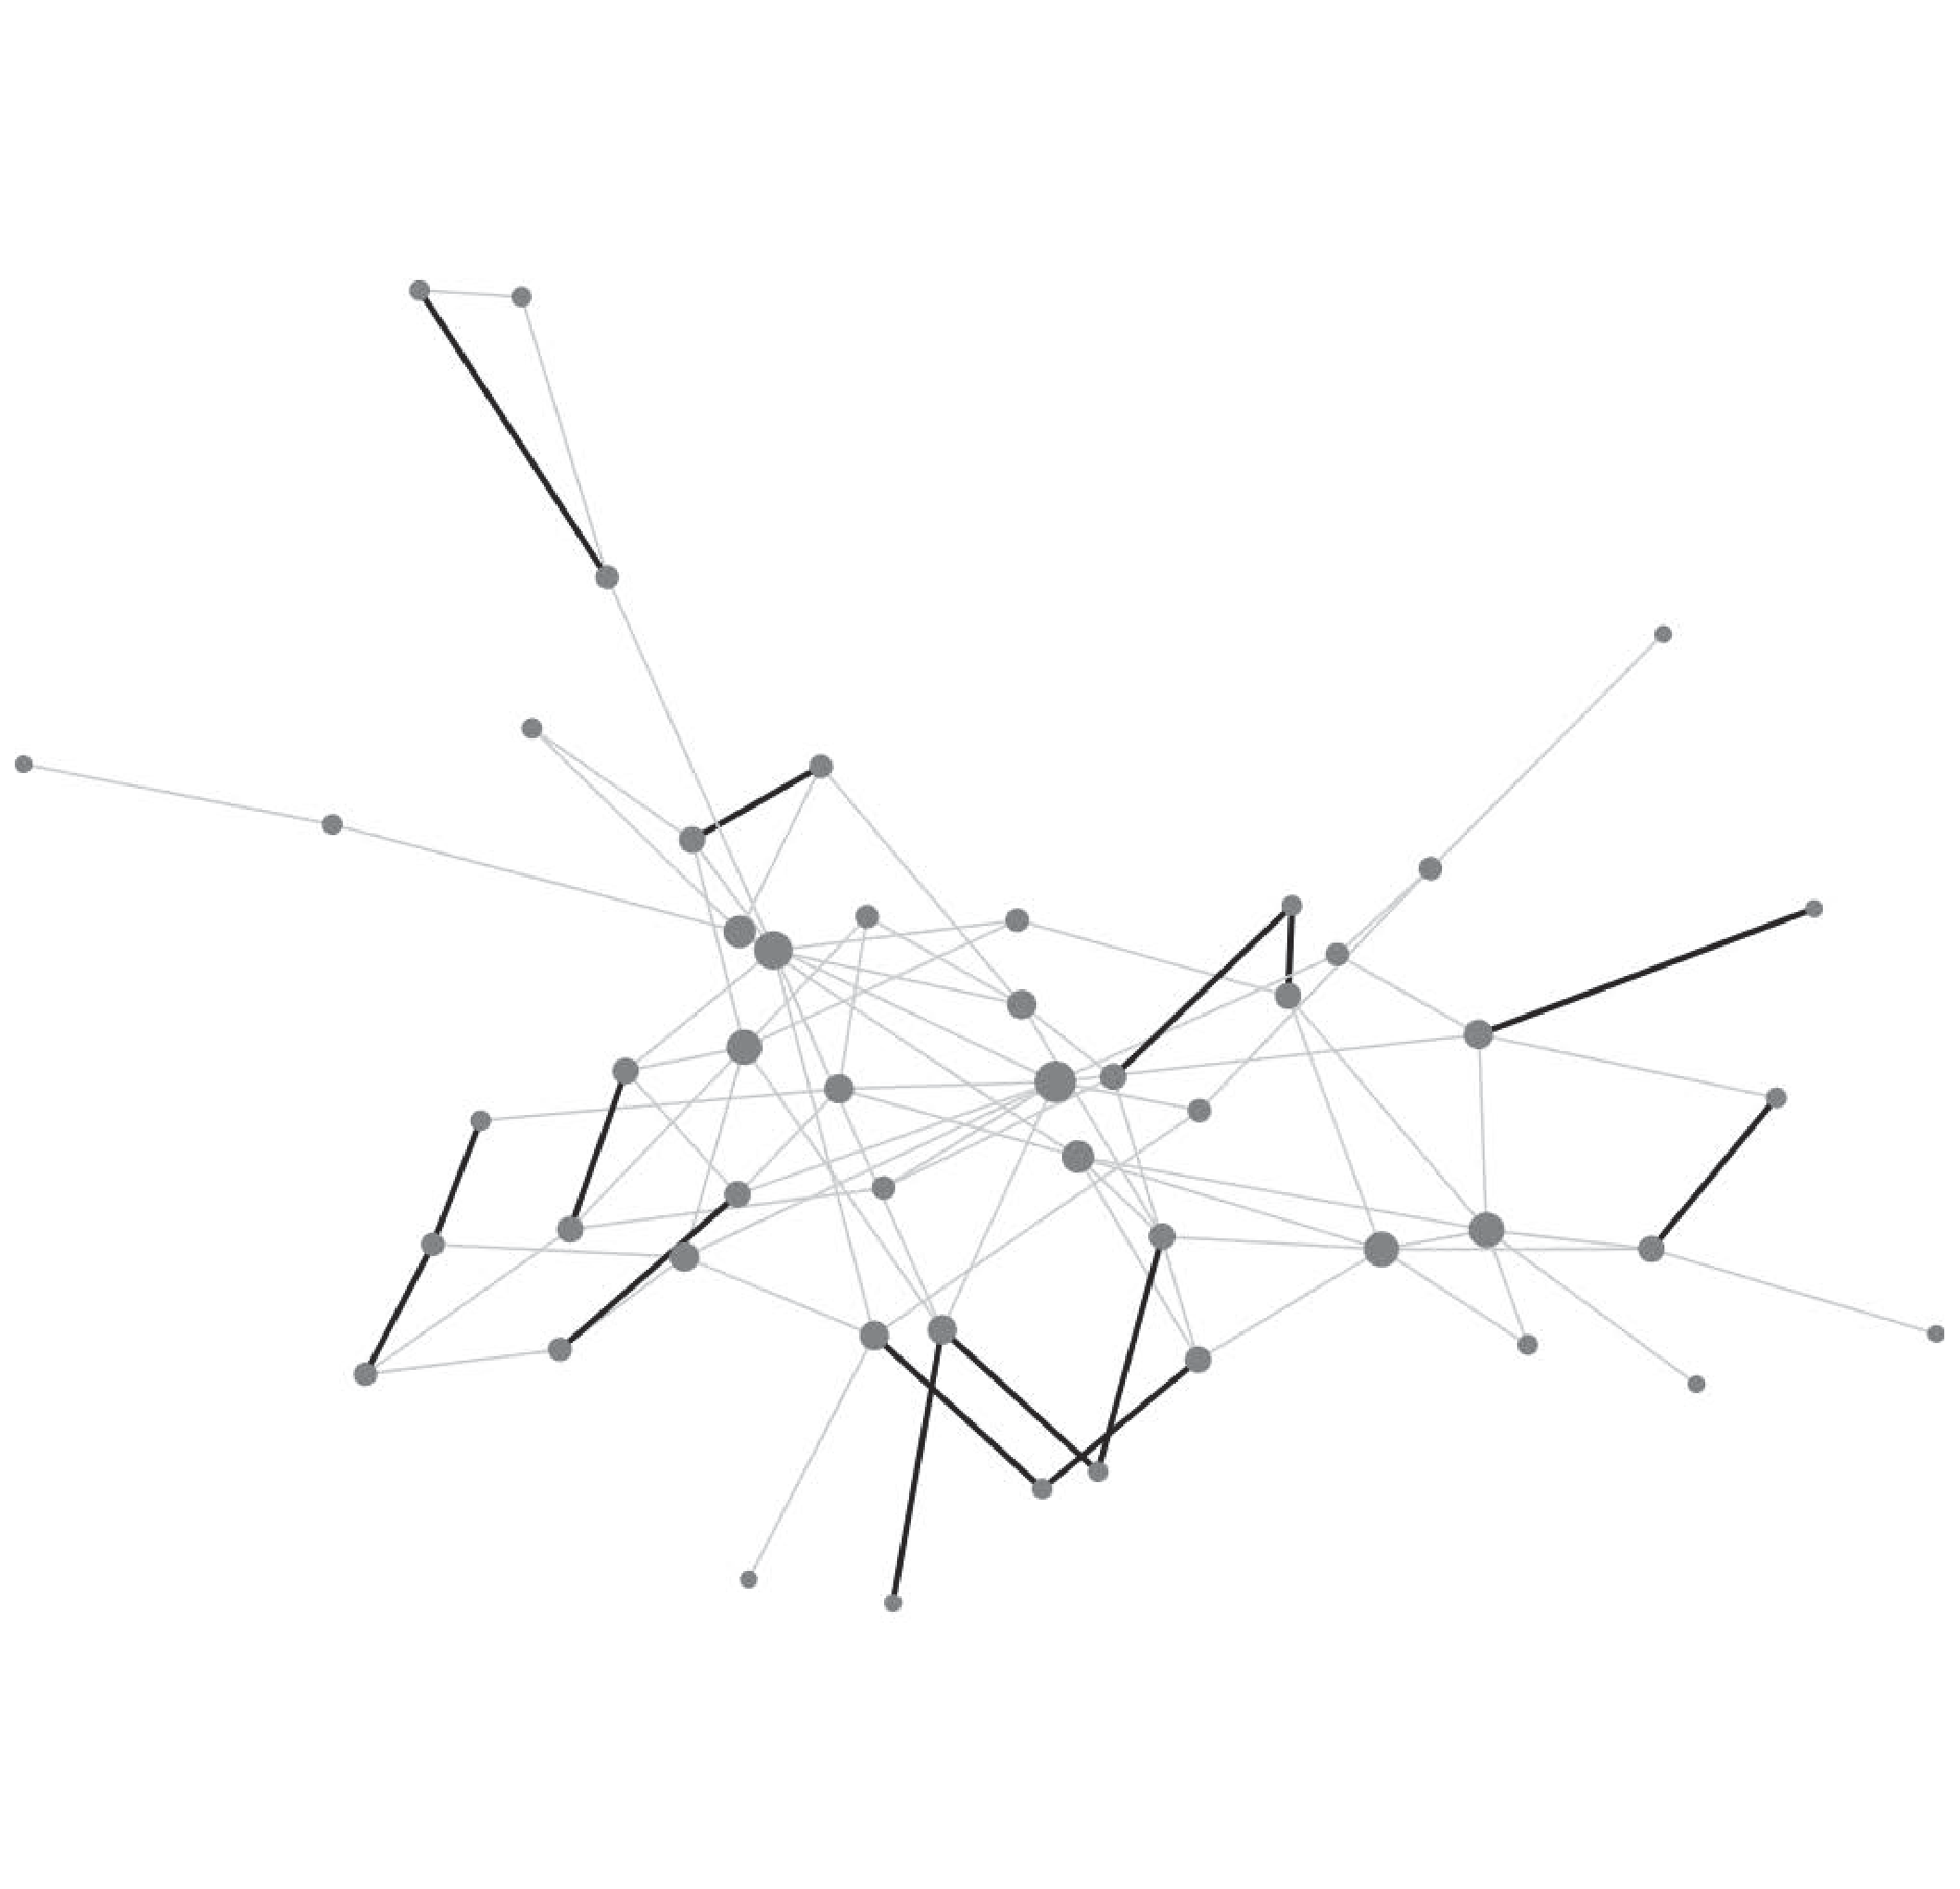
\epsfig{file=fig/SPA_15_50.eps,width=0.8\textwidth,height=0.2\textheight}}
  \centerline{(a) Sparse ($p=50, |E| = 88$)} \medskip
  \end{minipage} \medskip
\begin{minipage}[b]{.45\linewidth}
  \centering   \centerline{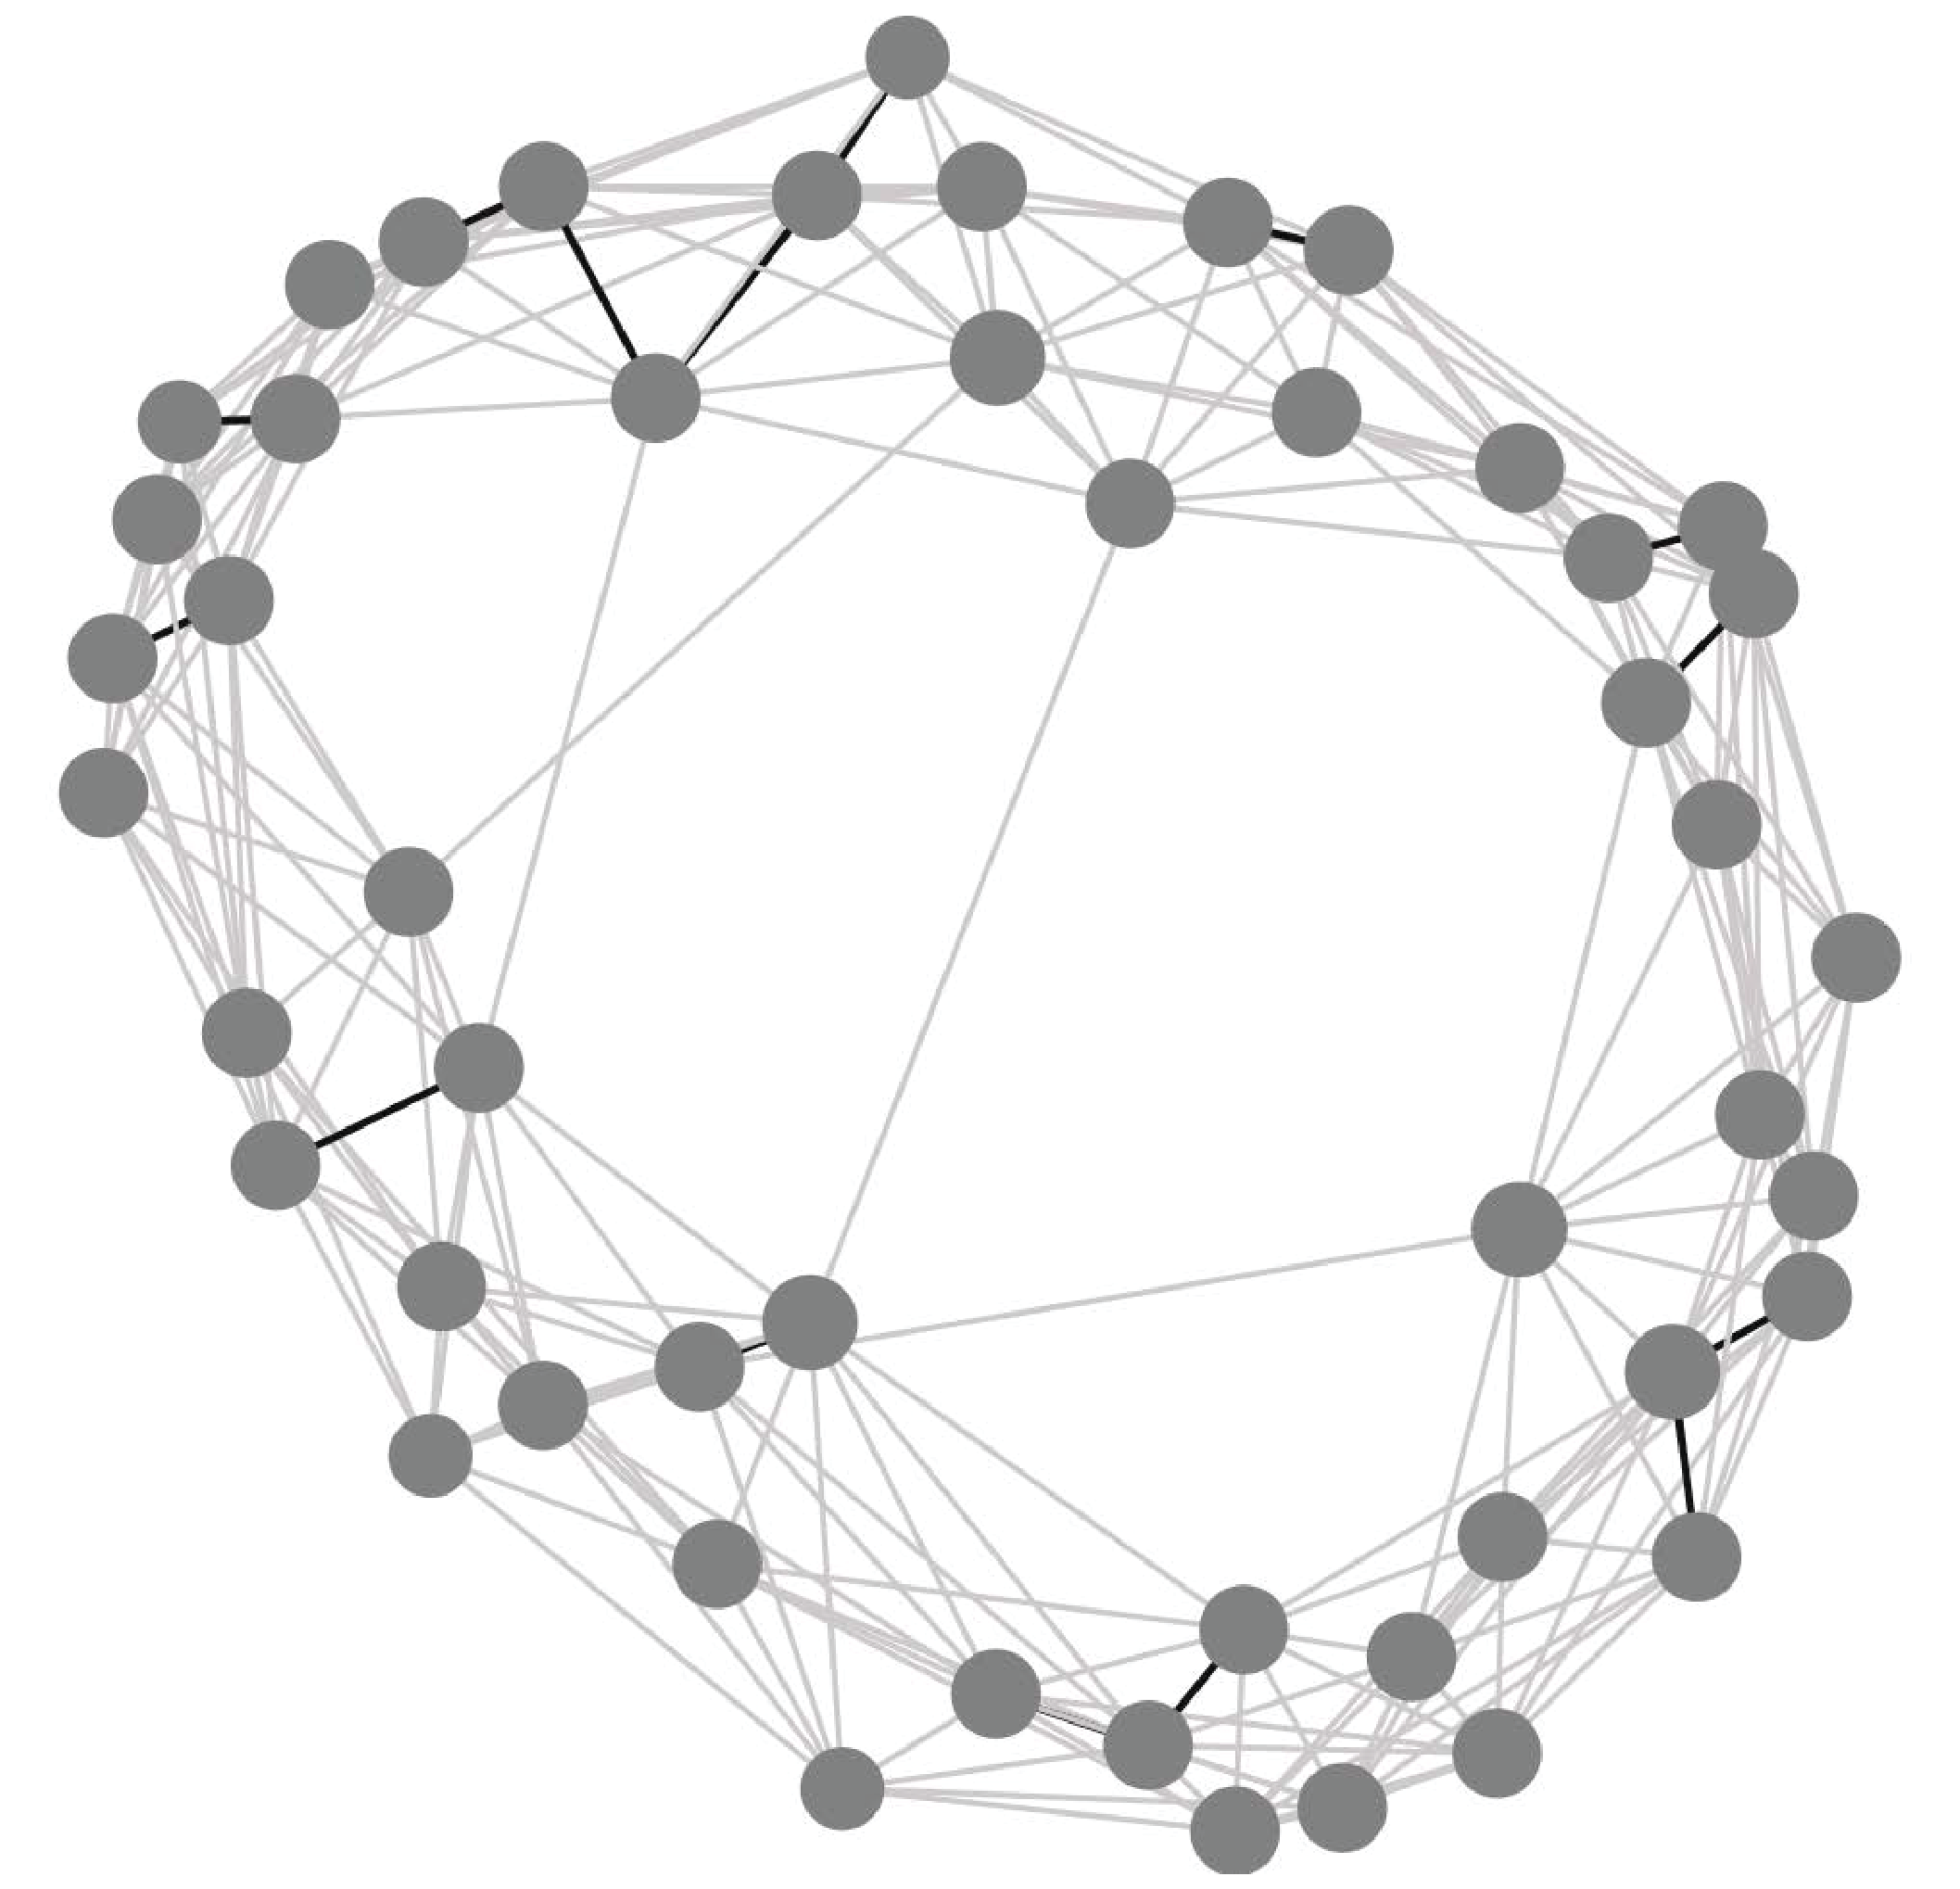
\epsfig{file=fig/DEN_15_50.eps,width=0.8\textwidth,height=0.2\textheight}}
  \centerline{(b) Dense ($p=50, |E| = 250$) } \medskip
\end{minipage}
\begin{minipage}[b]{.45\linewidth}
  \centering   \centerline{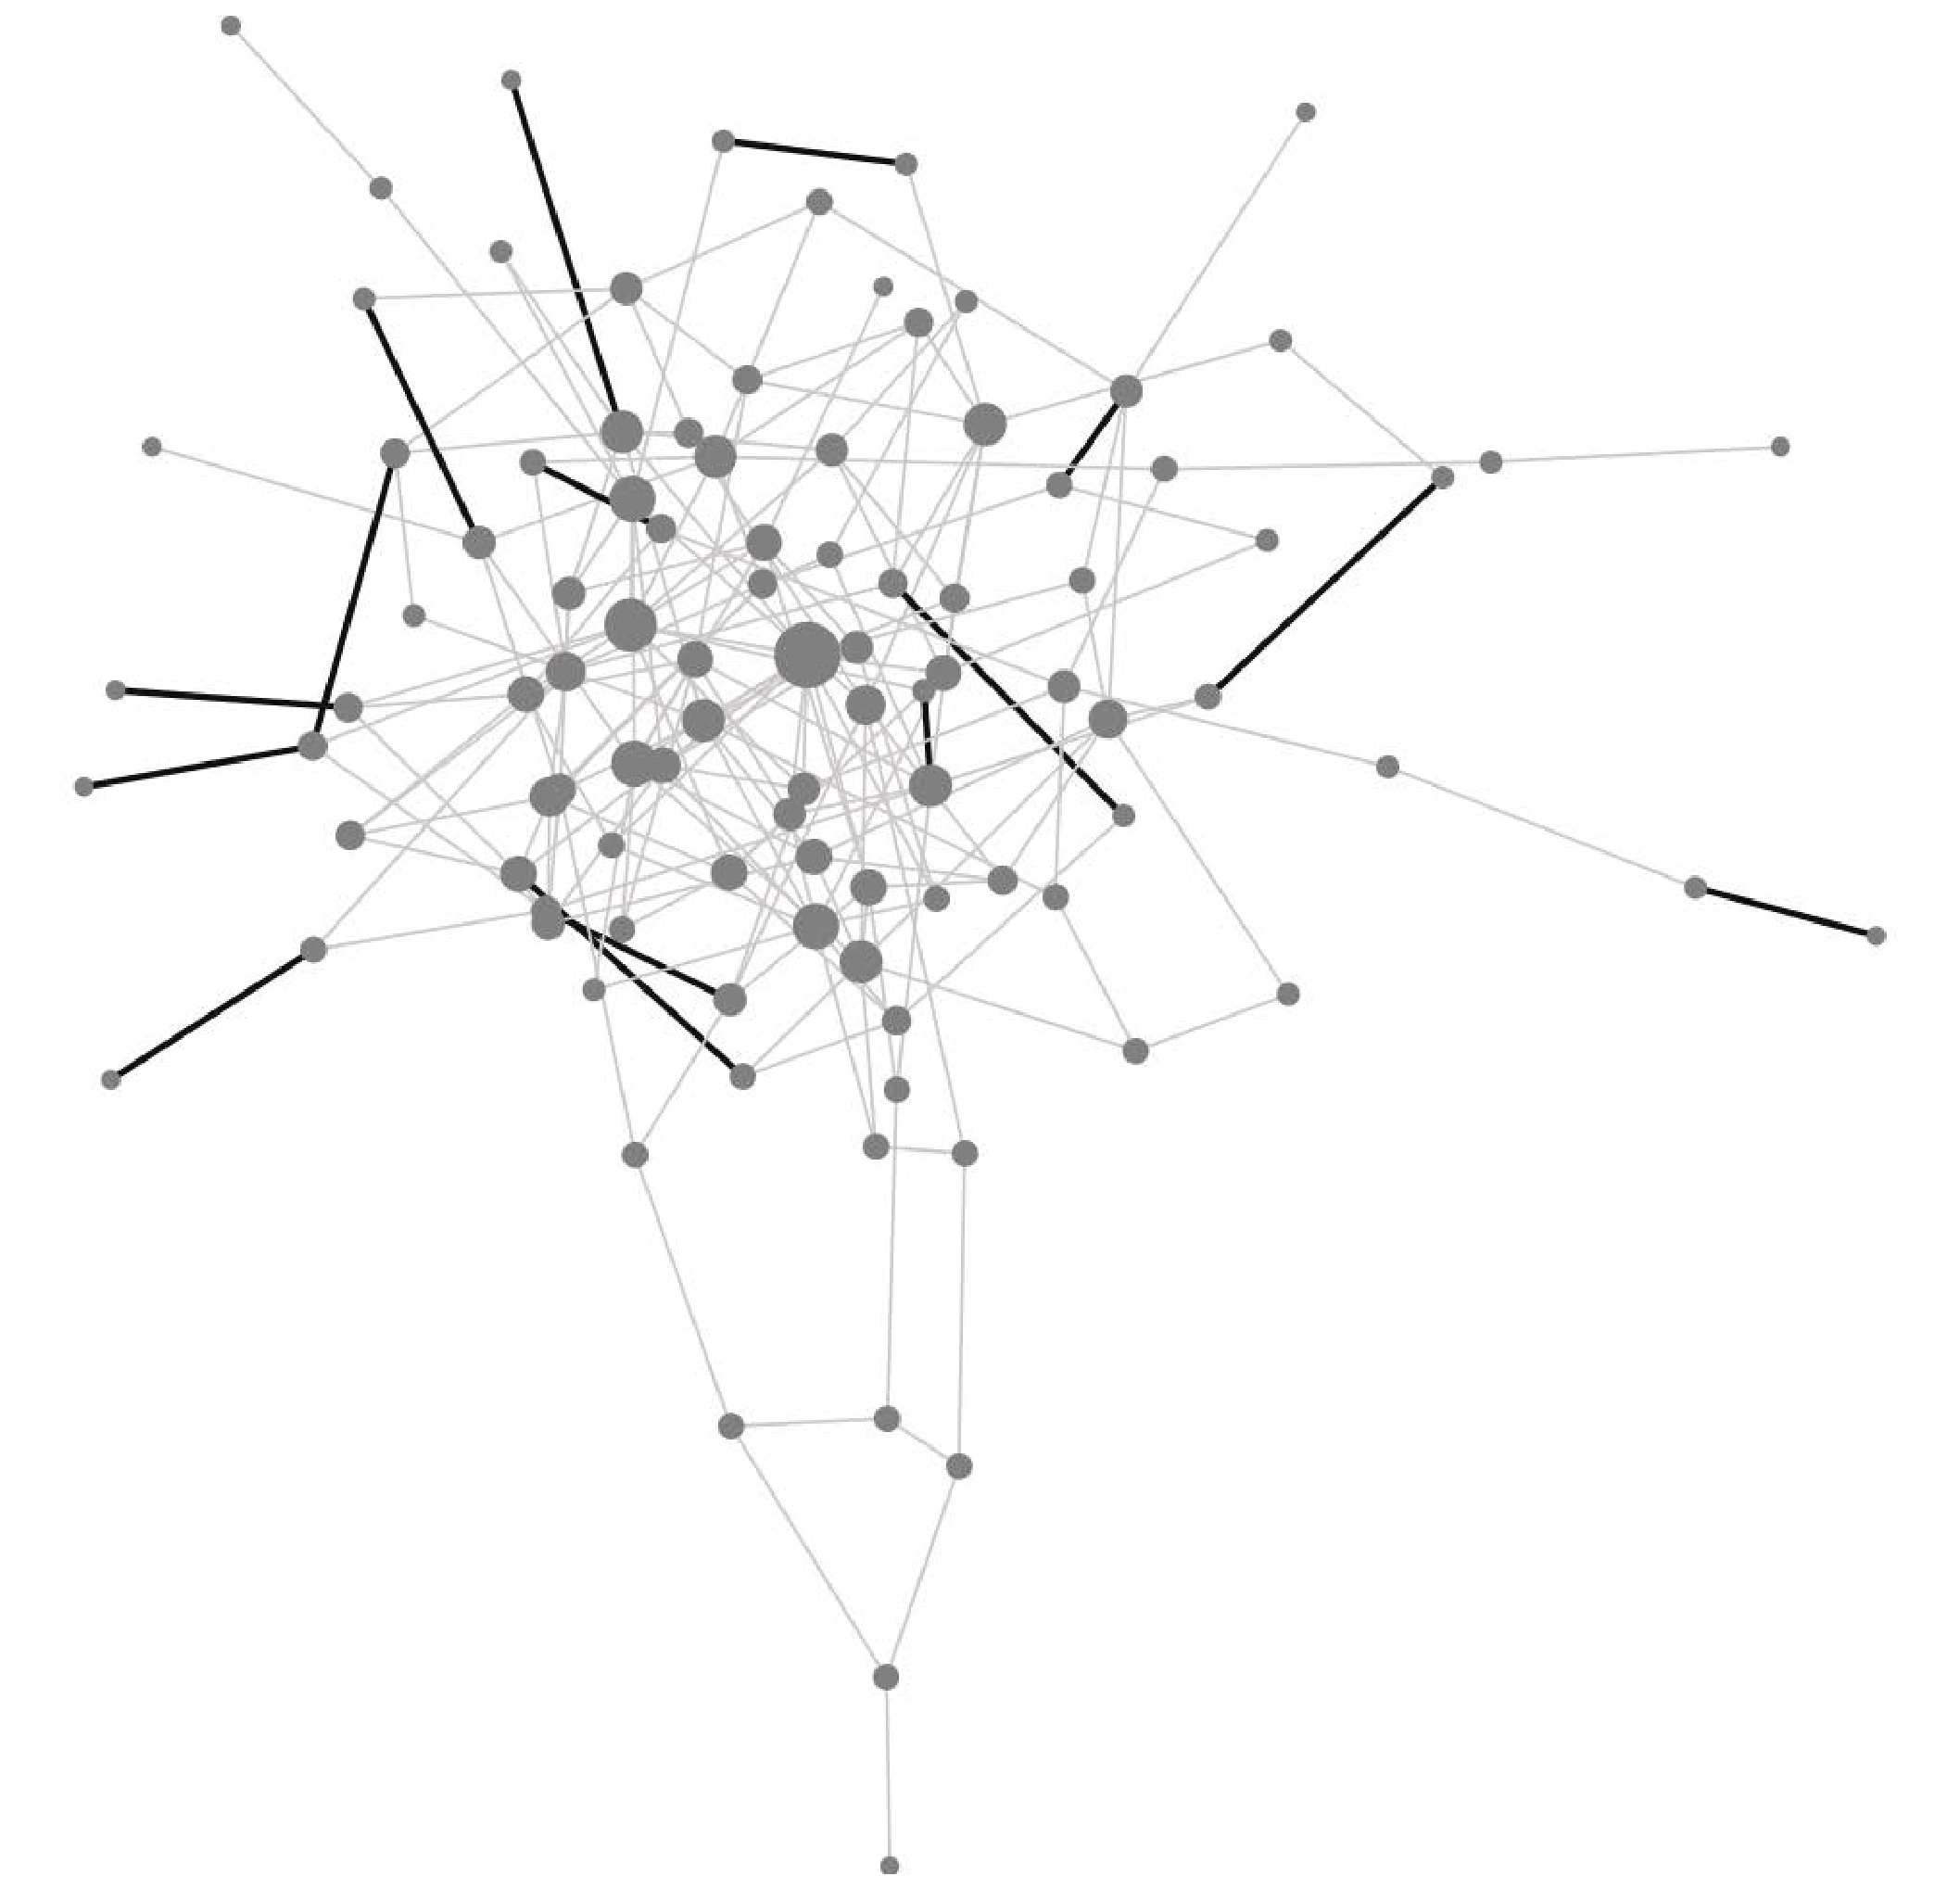
\epsfig{file=fig/SPA_15_100.eps,width=0.8\textwidth,height=0.2\textheight}}
  \centerline{(c) Sparse ($p=100, |E| = 205$)} \medskip
\end{minipage}
\begin{minipage}[b]{.45\linewidth}
  \centering   \centerline{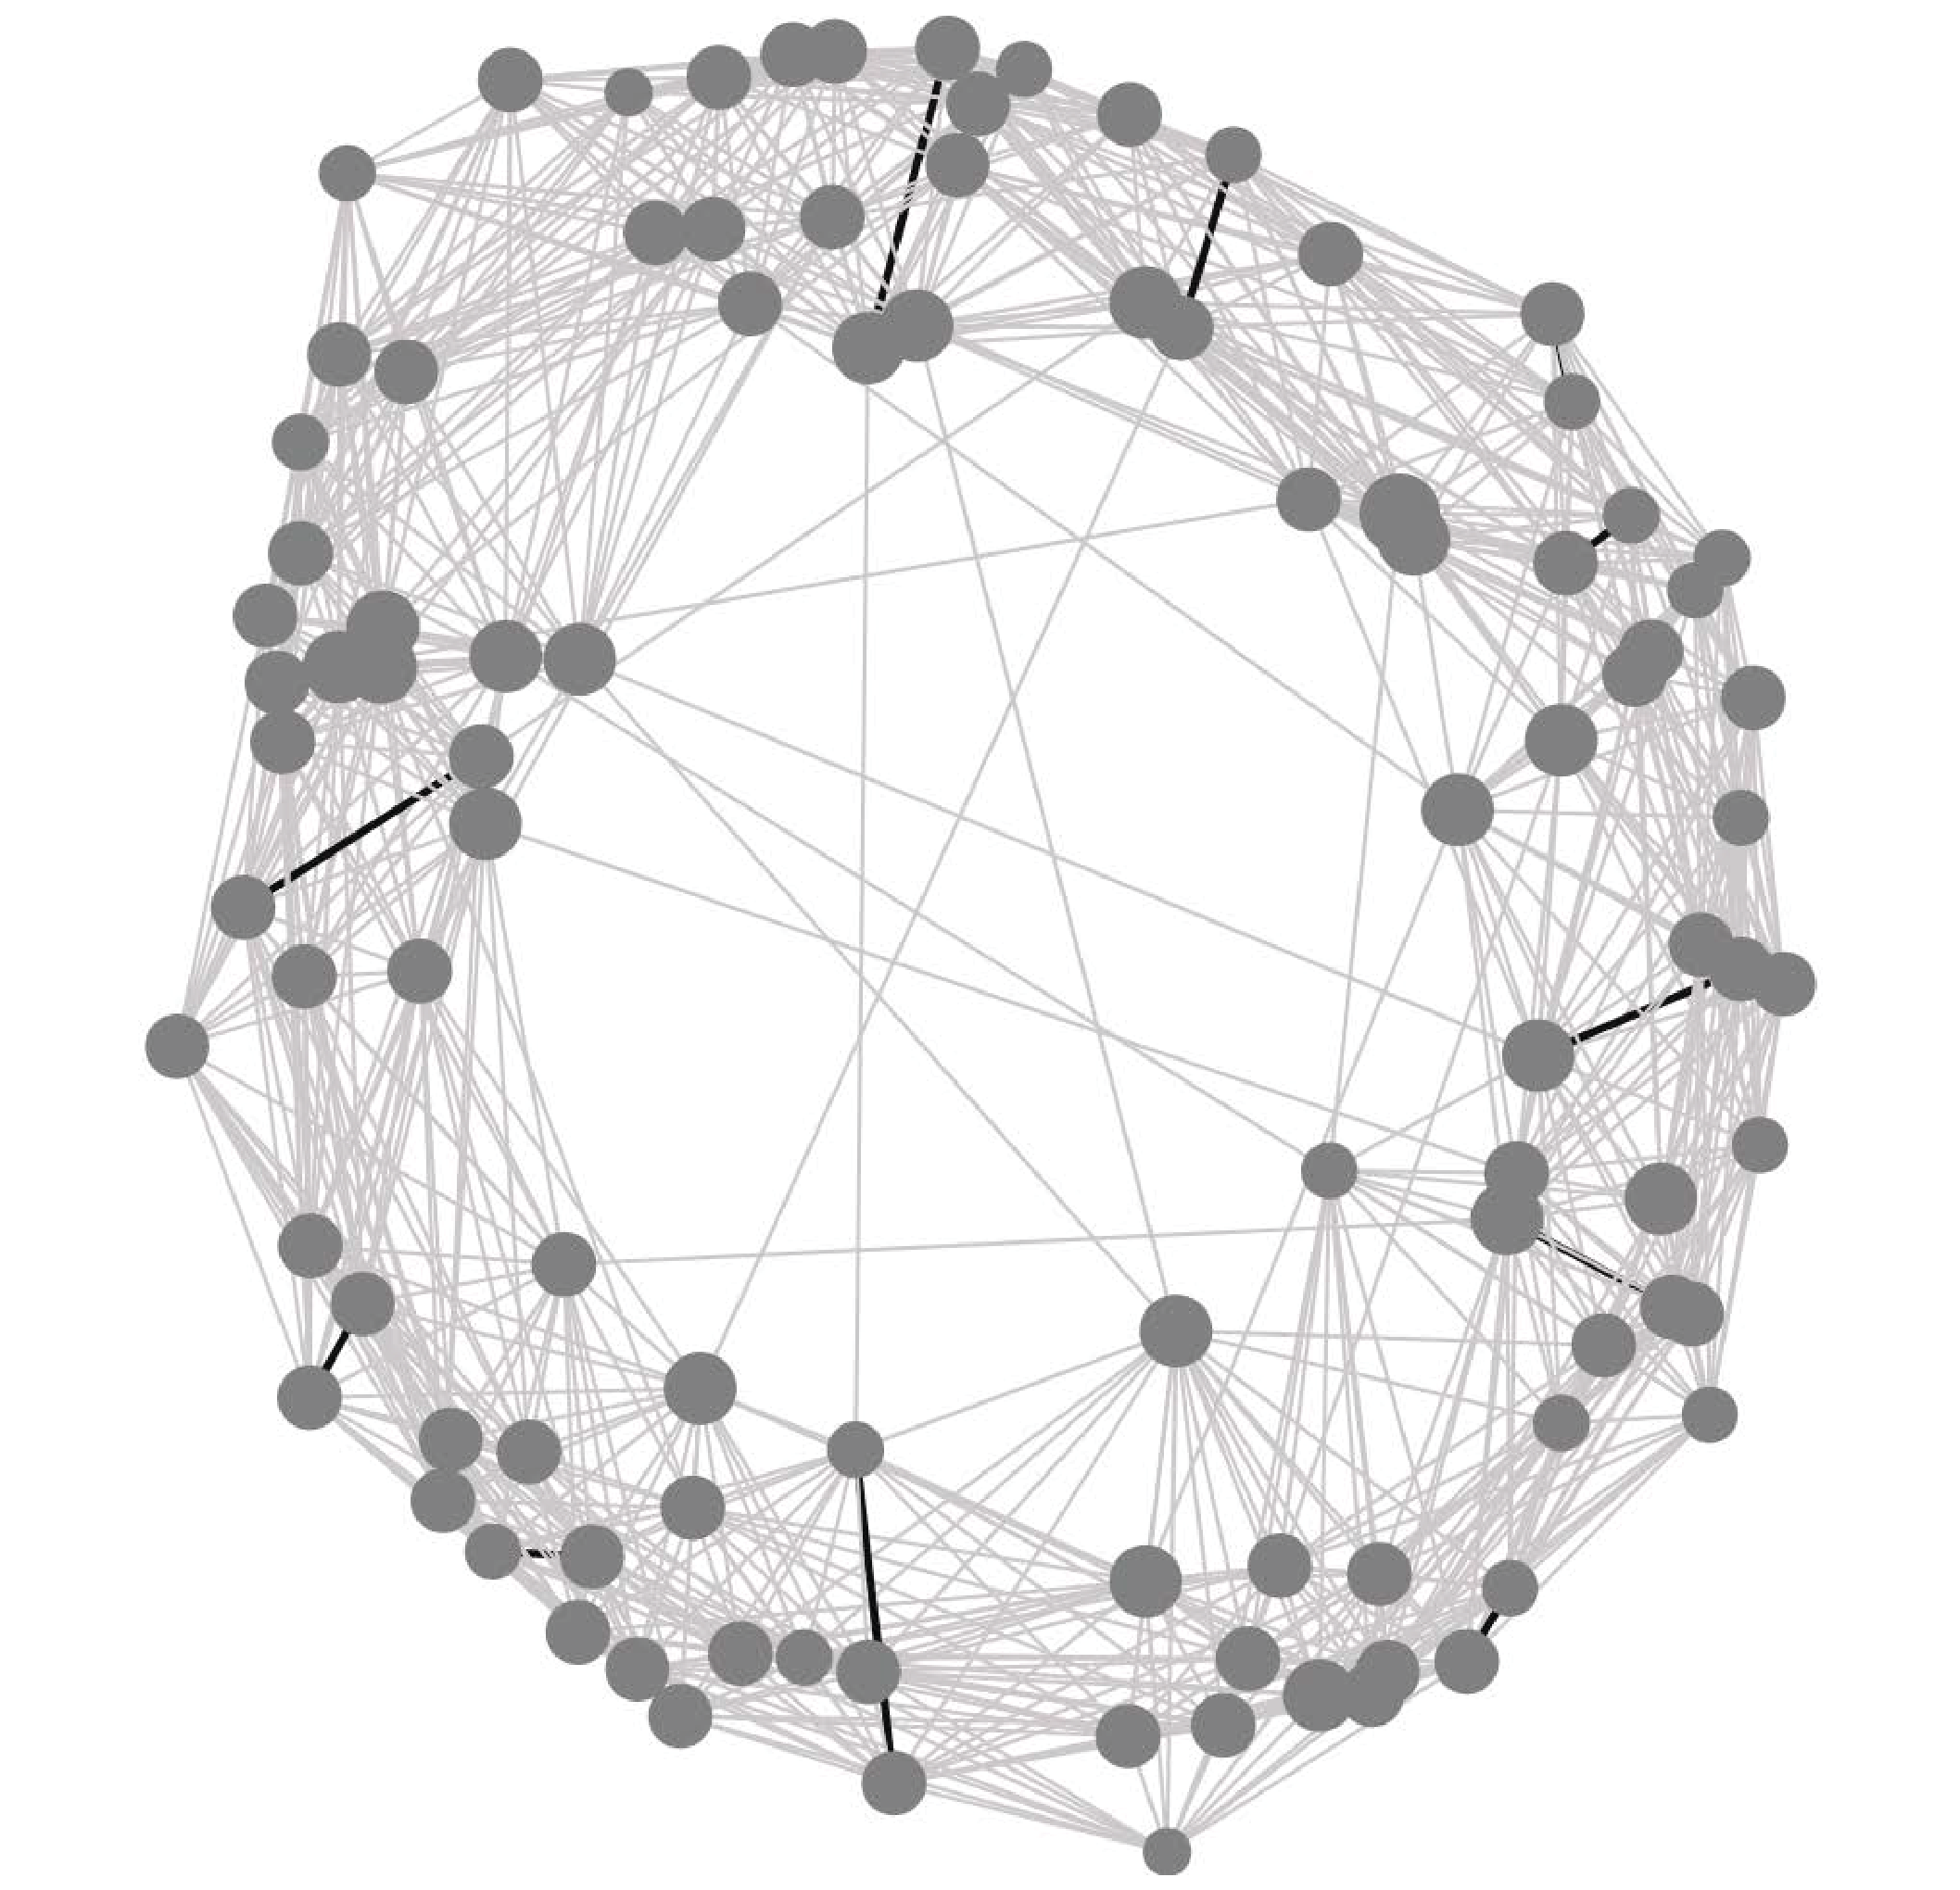
\epsfig{file=fig/DEN_15_100.eps,width=0.8\textwidth,height=0.2\textheight}}
  \centerline{(d) Dense  ($p=100, |E| = 1000$)} \medskip
\end{minipage}
\begin{minipage}[b]{.45\linewidth}
  \centering   \centerline{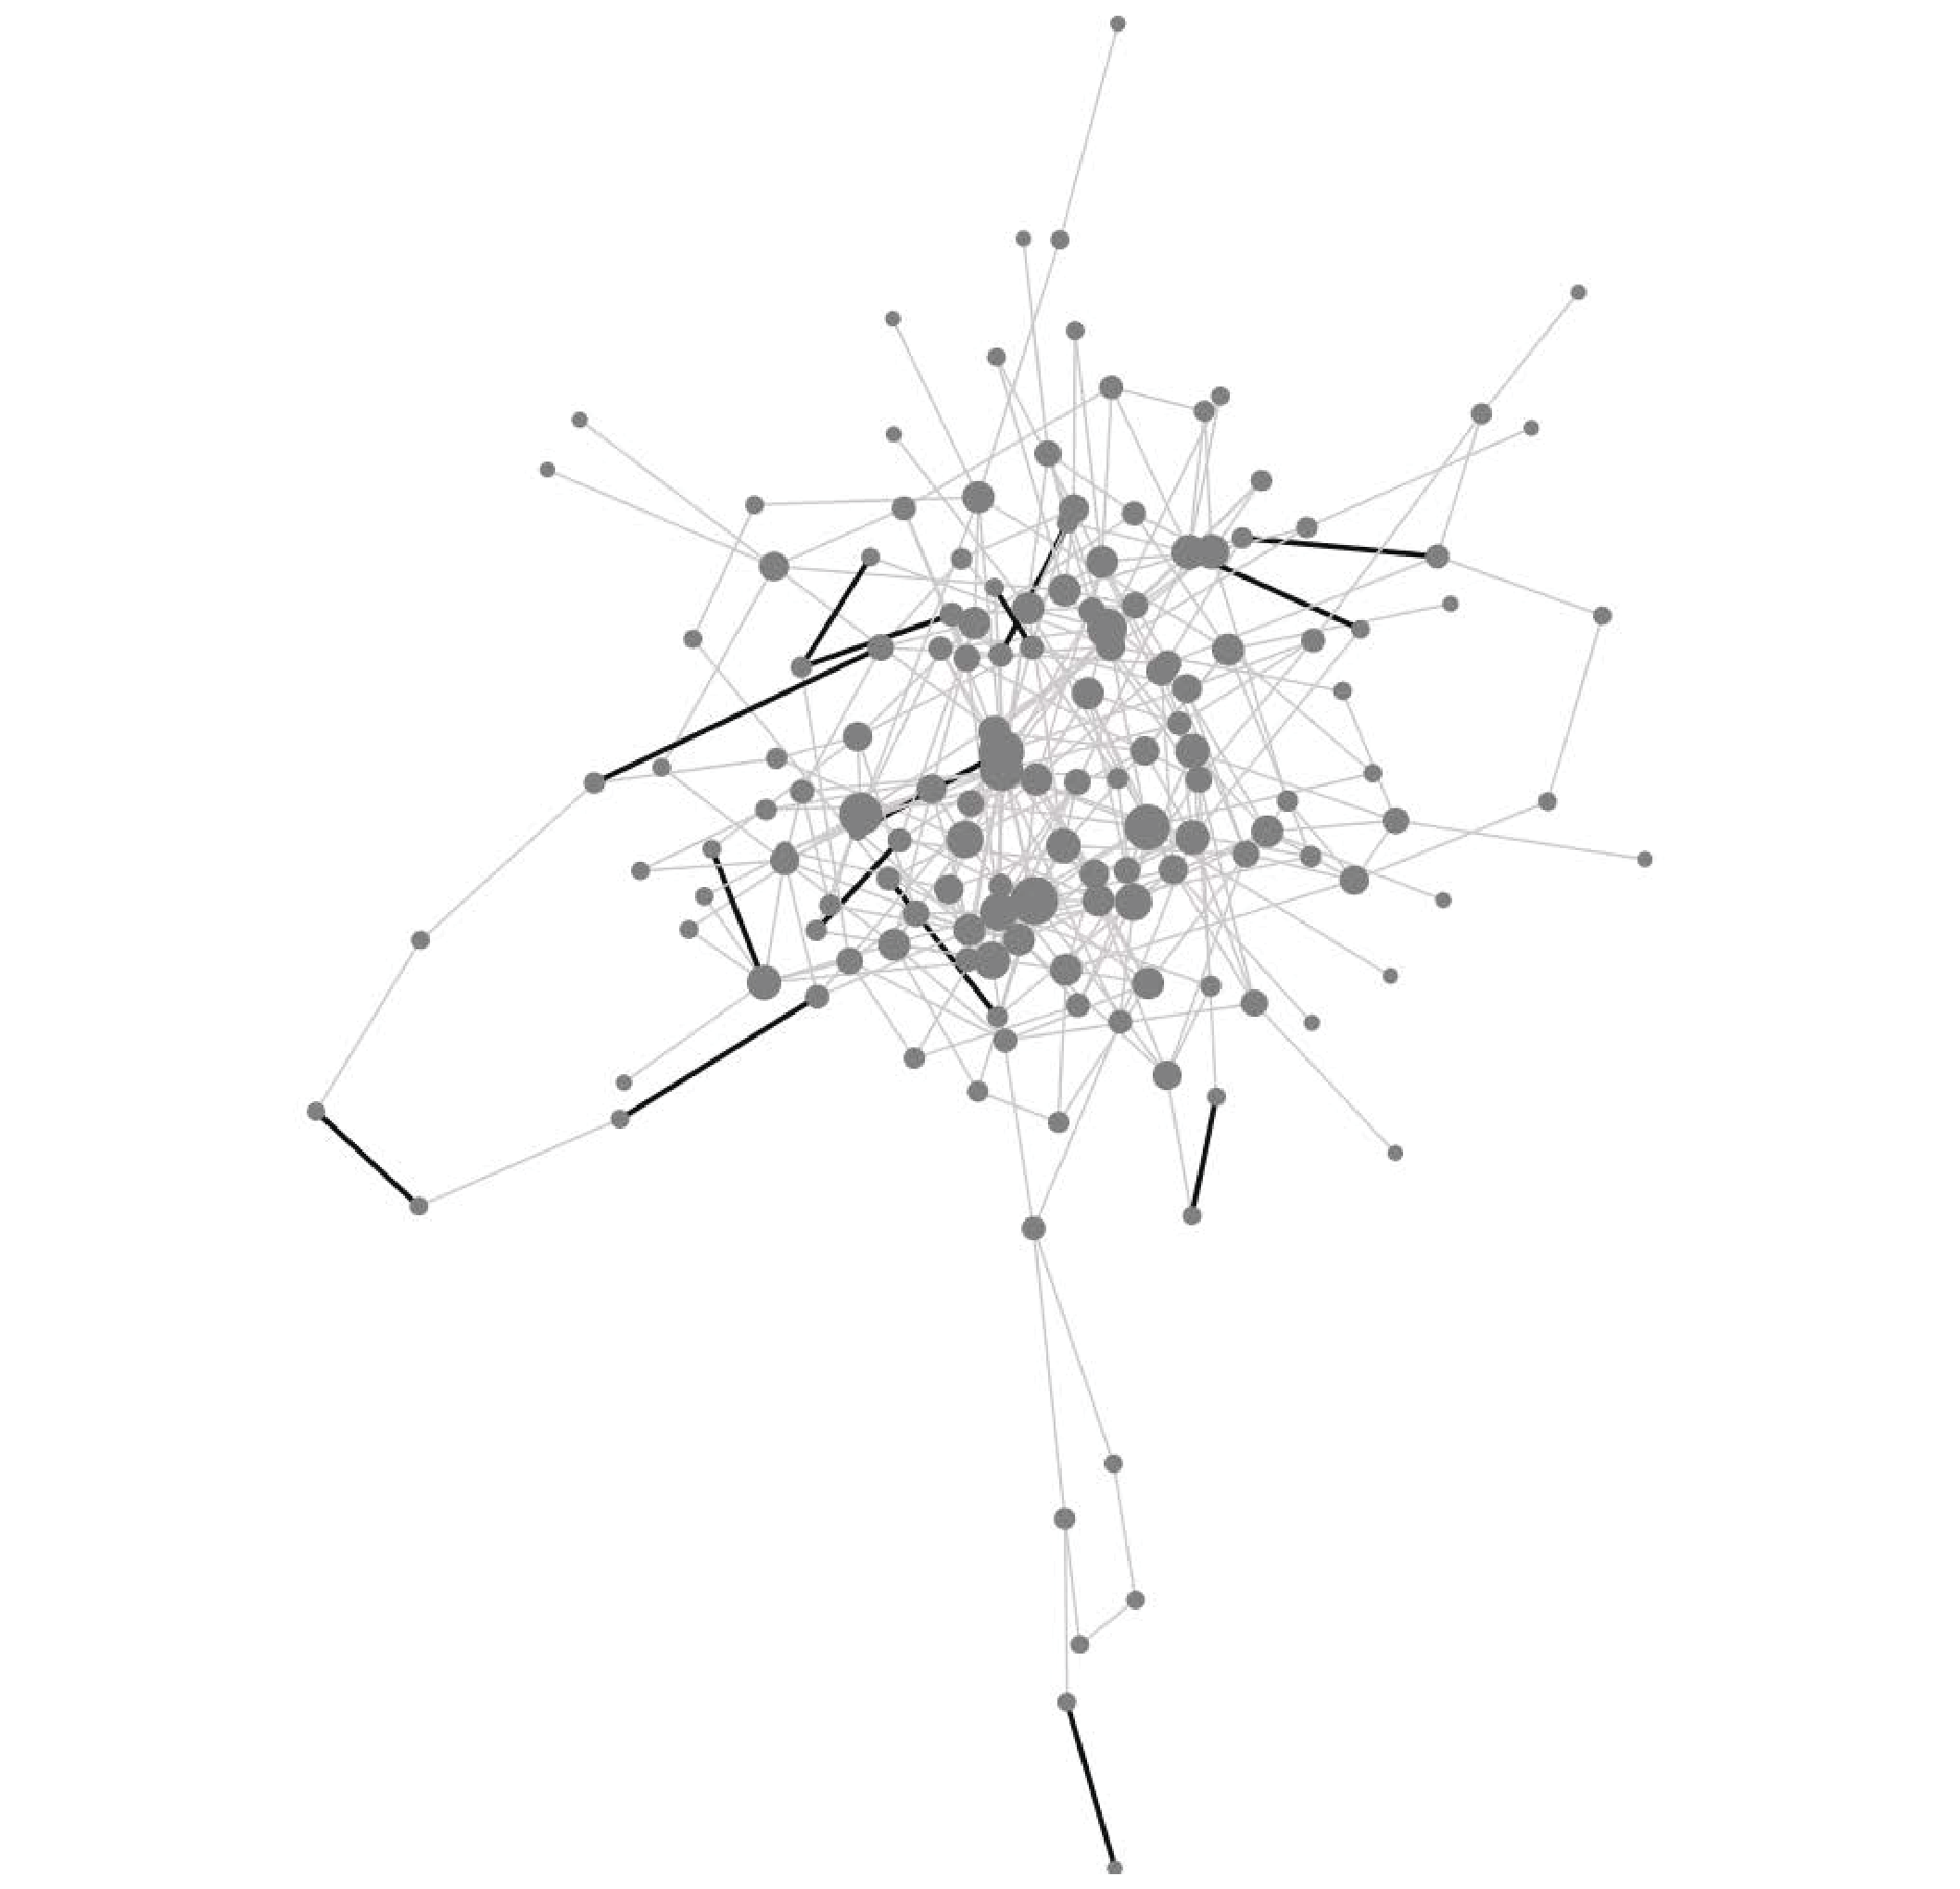
\epsfig{file=fig/SPA_15_150.eps,width=0.8\textwidth,height=0.2\textheight}}
  \centerline{(e) Sparse ($p=150, |E| = 327$) } \medskip
\end{minipage}
\begin{minipage}[b]{.45\linewidth}
  \centering   \centerline{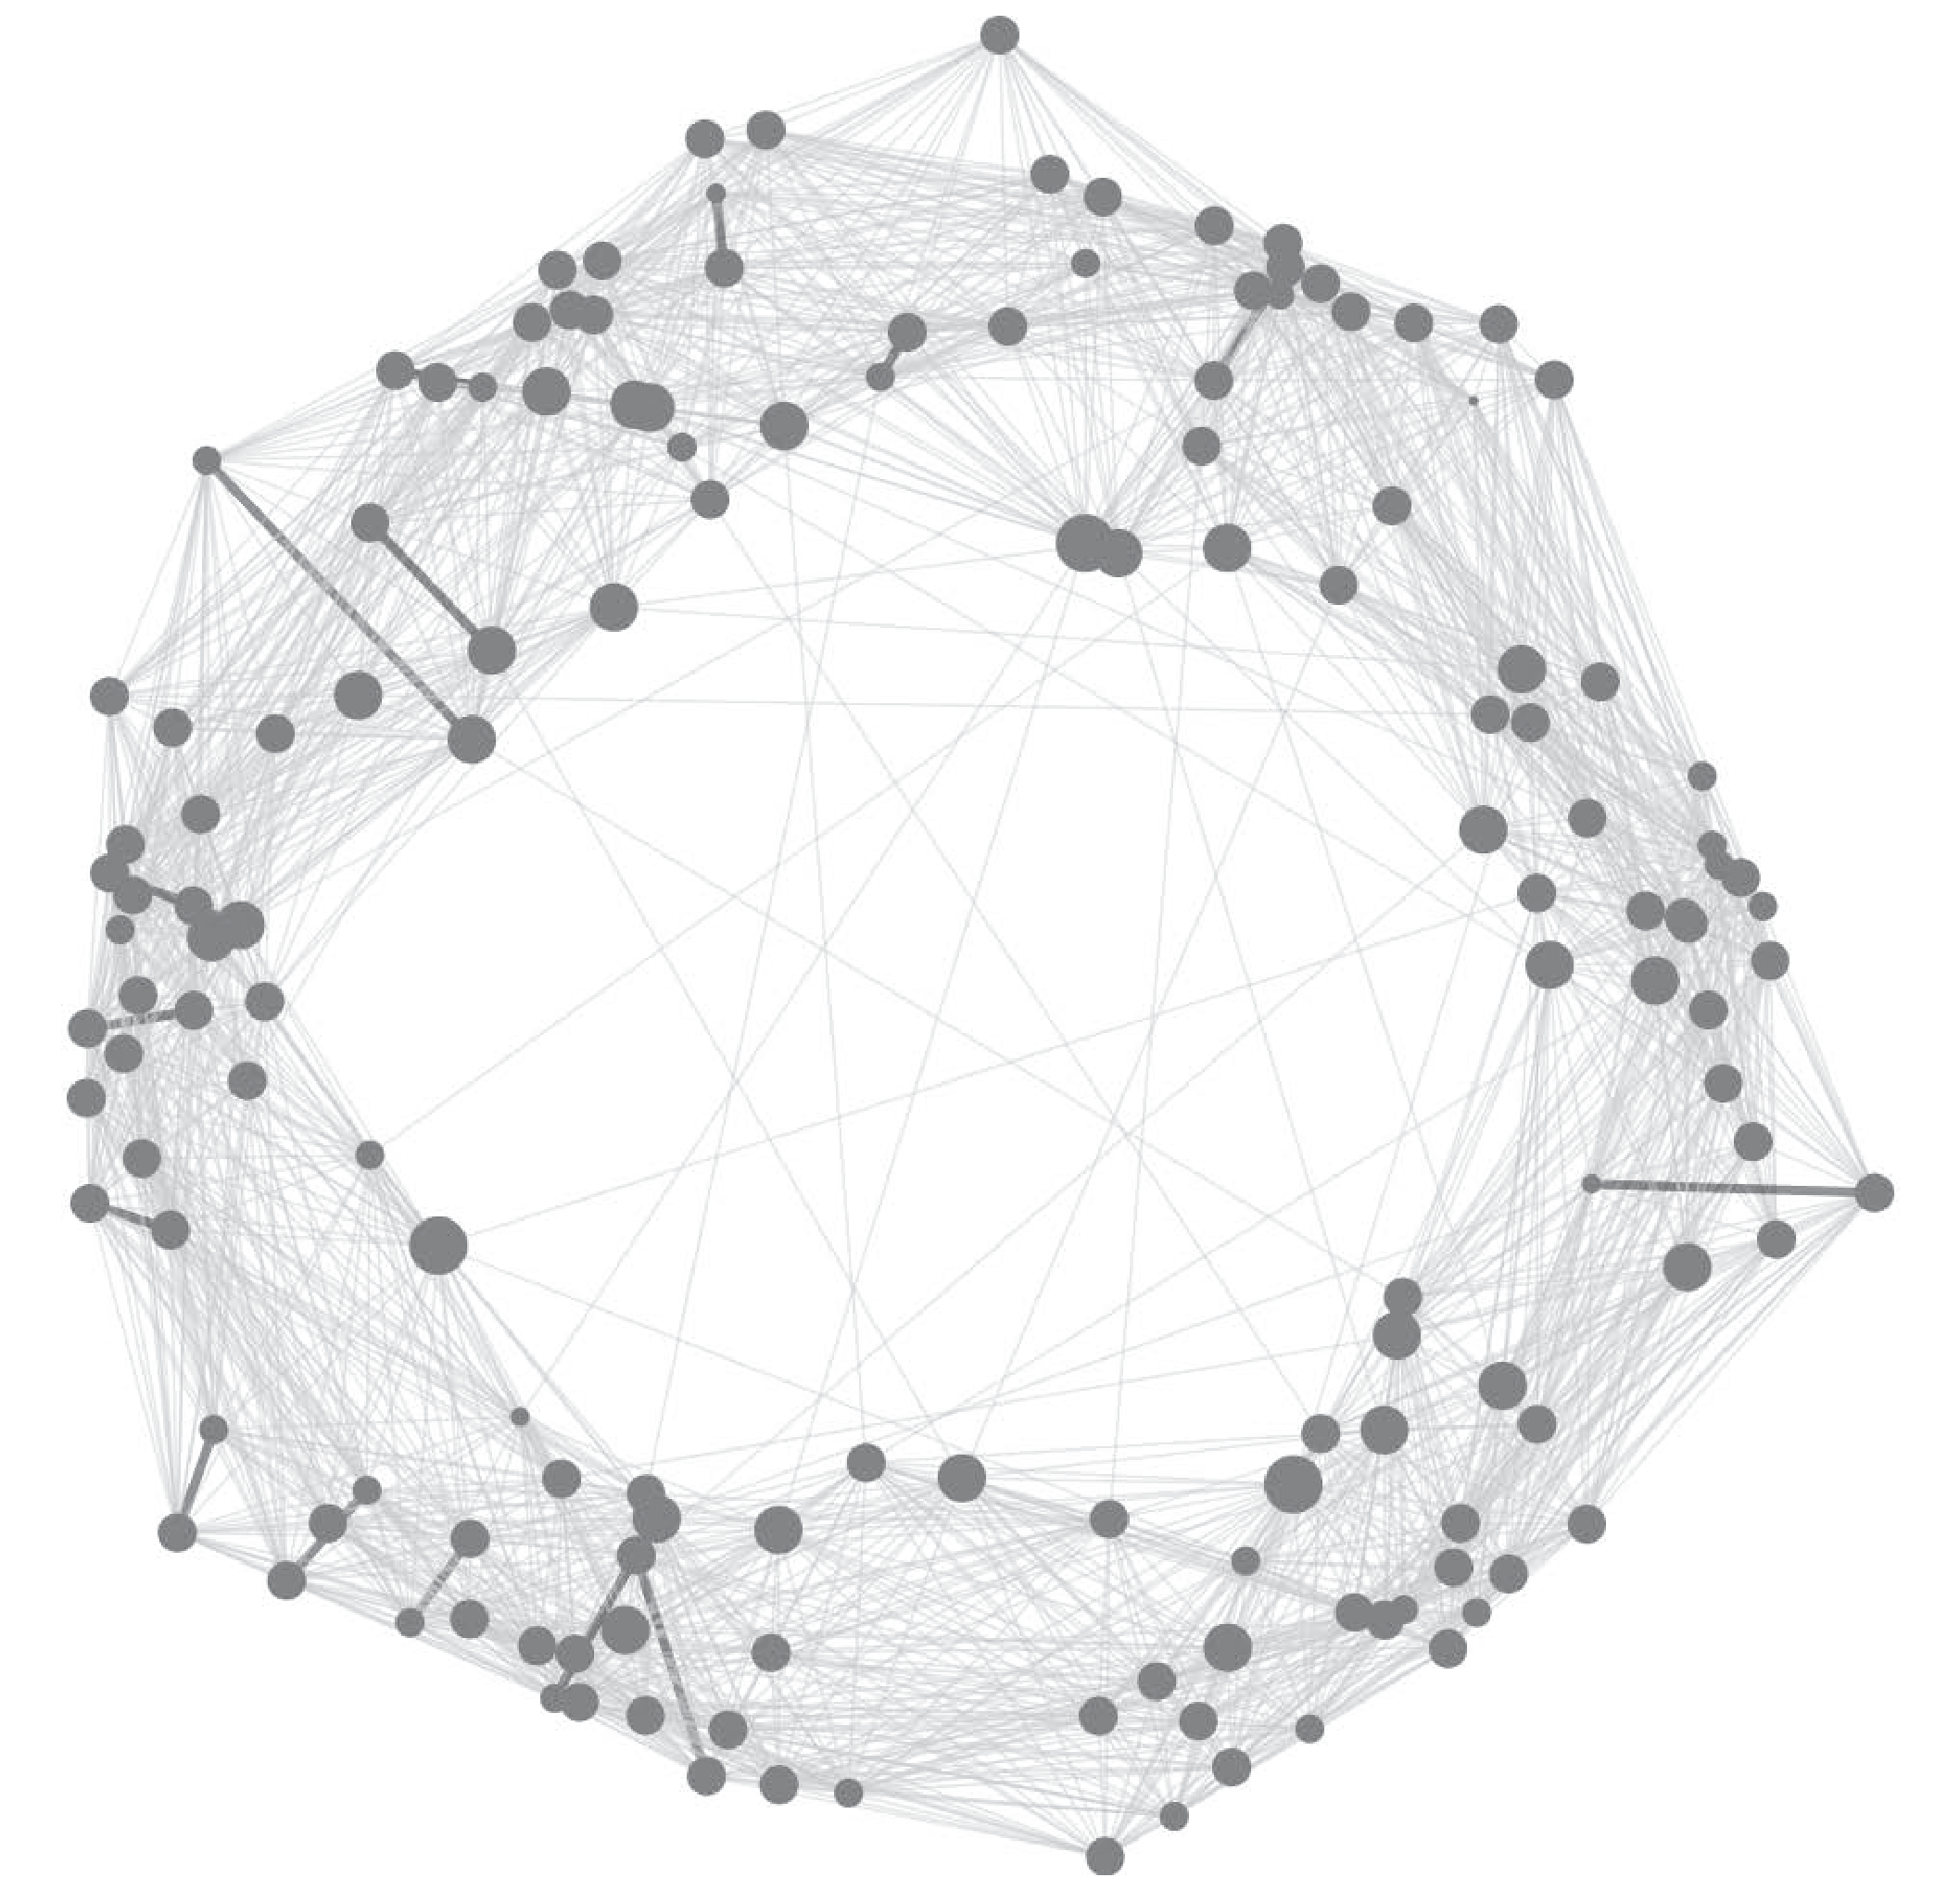
\epsfig{file=fig/DEN_15_150.eps,width=0.8\textwidth,height=0.2\textheight}}
  \centerline{(f) Dense  ($p=150, |E| = 2250$)} \medskip
\end{minipage}
\caption{Examples of sparse in the left panels and dense networks 
in the right panels for each case in the numerical study.
Black lines denote differential edges between two networks and 
gray lines denote edges.}
\end{center}
\end{figure}


\begin{figure}[htb!] %\label{}
\begin{center} \medskip
\begin{minipage}[b]{.48\linewidth}
  \centering   \centerline{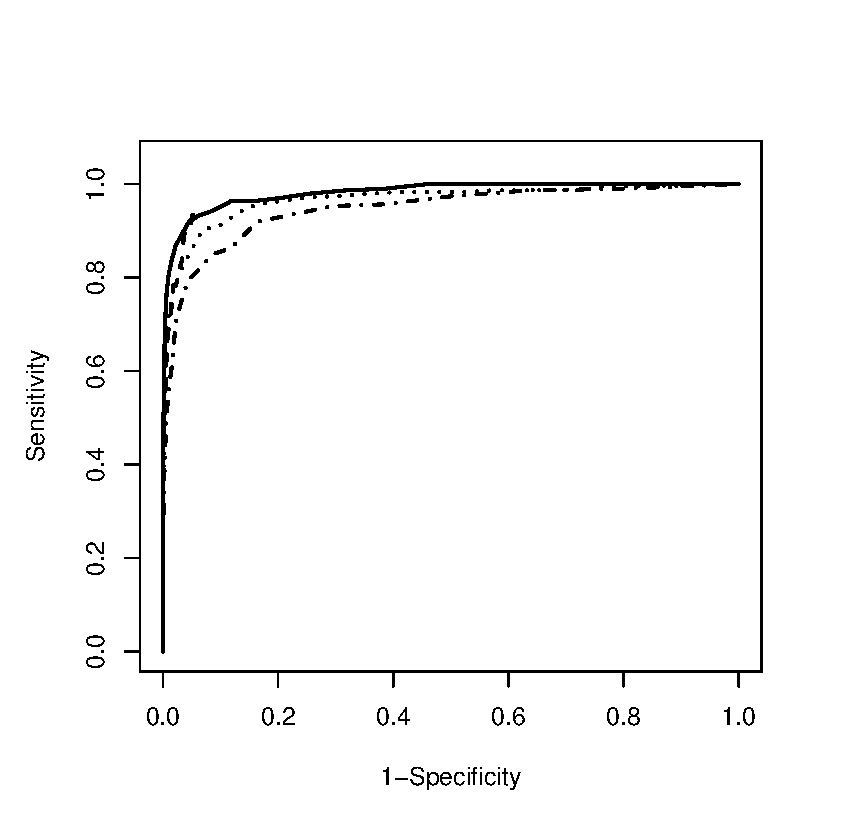
\epsfig{file=fig/AUC_1.eps,width=0.9\textwidth,height=0.35\textheight}}
  \centerline{(a) {(\bf C1)} Sparse, Structure}
\end{minipage} \medskip
\begin{minipage}[b]{.48\linewidth}
  \centering   \centerline{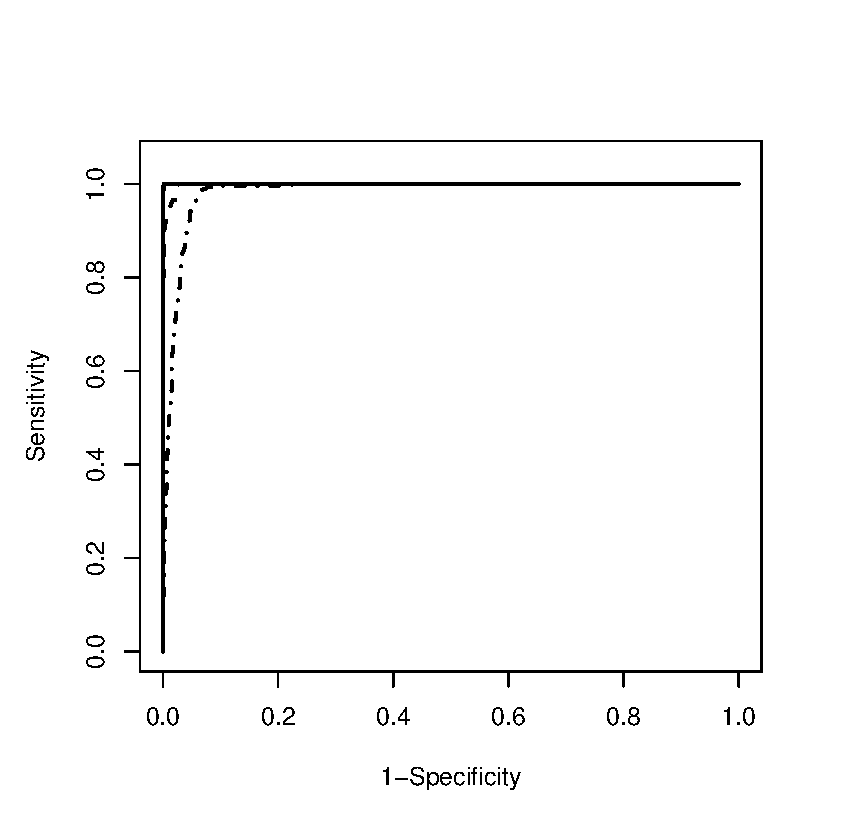
\epsfig{file=fig/AUC_4.eps,width=0.9\textwidth,height=0.35\textheight}}
  \centerline{(b) {(\bf C2)} Sparse, Direction }
\end{minipage}
\medskip
\begin{minipage}[b]{.48\linewidth}
  \centering   \centerline{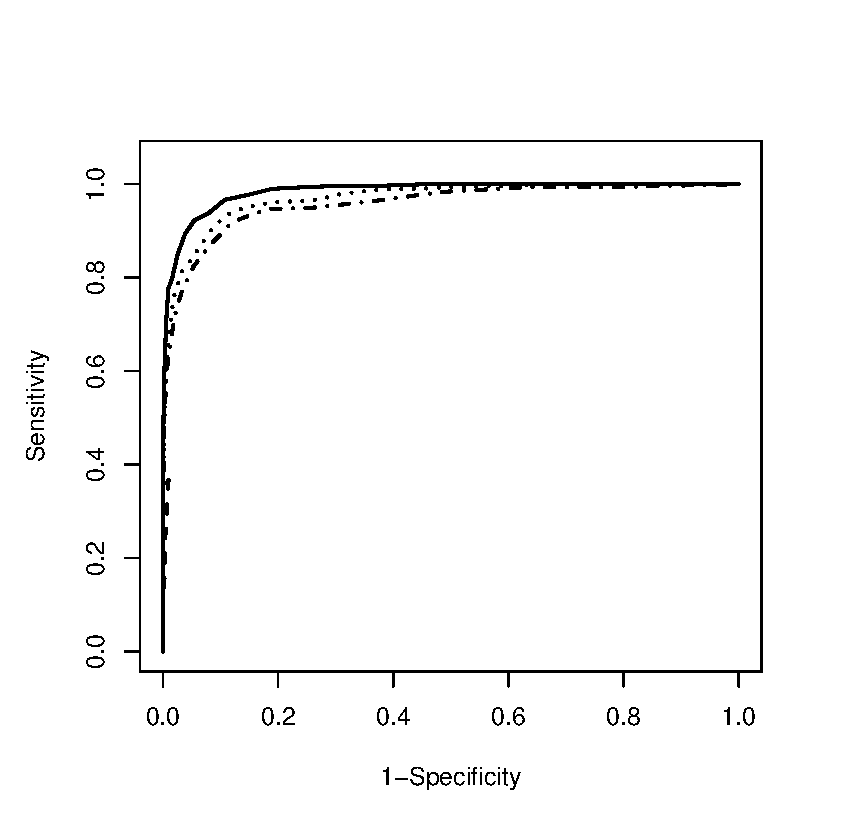
\epsfig{file=fig/AUC_7.eps,width=0.9\textwidth,height=0.35\textheight}}
  \centerline{(c) {(\bf C3)} Dense, Structure}
\end{minipage}
\begin{minipage}[b]{.48\linewidth}
  \centering   \centerline{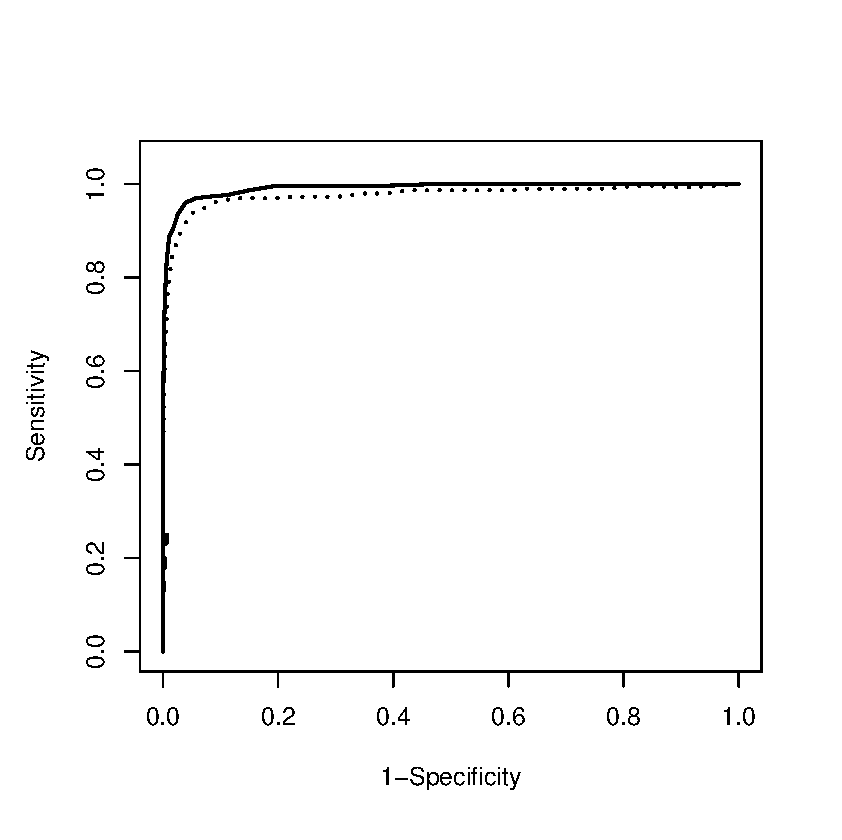
\epsfig{file=fig/AUC_8.eps,width=0.9\textwidth,height=0.35\textheight}}
  \centerline{(d) {(\bf C4)} Dense, Direction}
\end{minipage}
\caption{Receive operating characteristics curves for the sparse and 
dense networks ($p=50, n=100$) in separate panels for each scenario. 
Solid line represents JPACE($\lambda_1^*$), dashed line represents
JGL($\lambda_1^*$), dotted line represents JGL($\lambda_1=0$), 
and dot-dashed line represents DDN, where $\lambda_1^*$ denote 
the chosen $\lambda_1$ by the AIC in the numerical study.}
\end{center}
\end{figure}



\begin{figure}[htb!] %\label{}
\begin{center} \medskip
\begin{minipage}[b]{.48\linewidth}
  \centering   \centerline{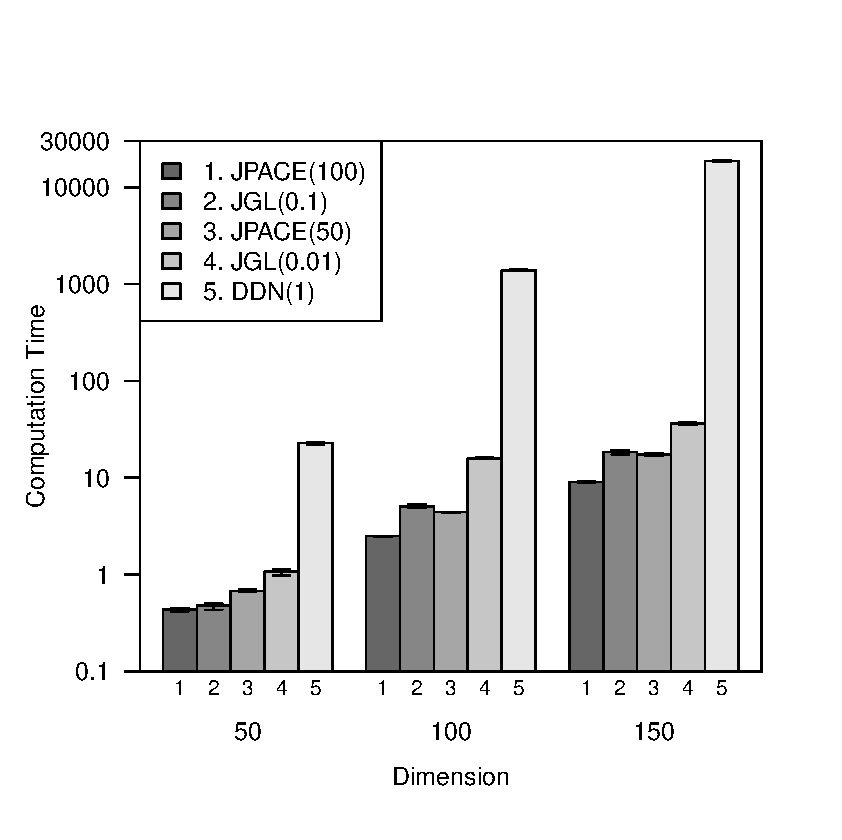
\epsfig{file=fig/time_spa_a.eps,width=0.9\textwidth,height=0.35\textheight}}
  \centerline{(a) Sparse, Structure}
\end{minipage} \medskip
\begin{minipage}[b]{.48\linewidth}
  \centering   \centerline{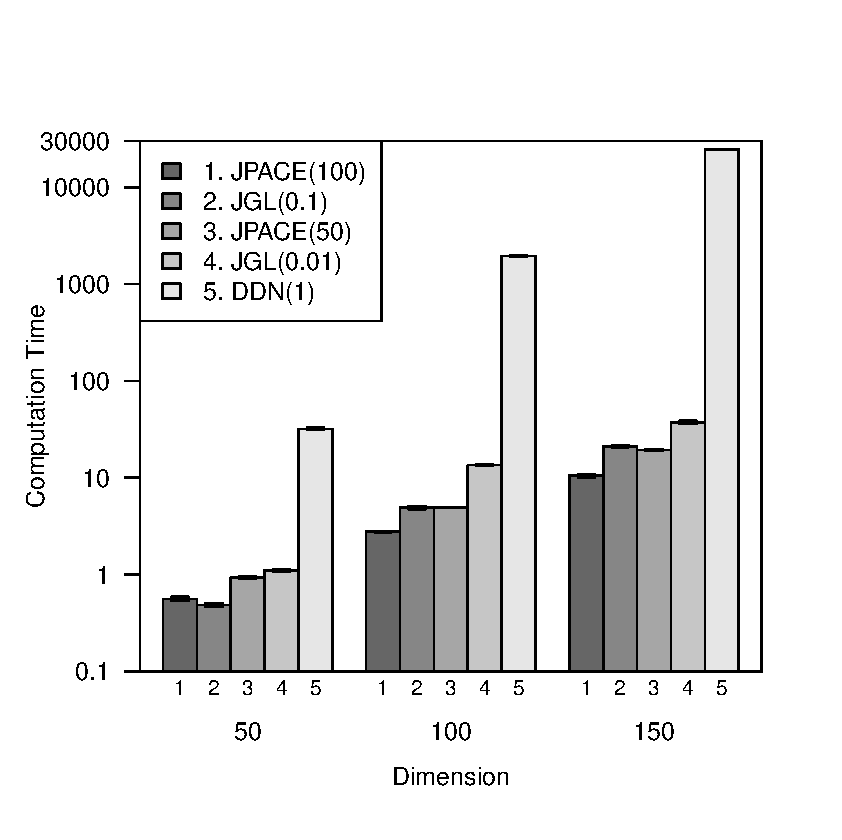
\epsfig{file=fig/time_spa_b.eps,width=0.9\textwidth,height=0.35\textheight}}
  \centerline{(b) Sparse, Direction }
\end{minipage}
\medskip
\begin{minipage}[b]{.48\linewidth}
  \centering   \centerline{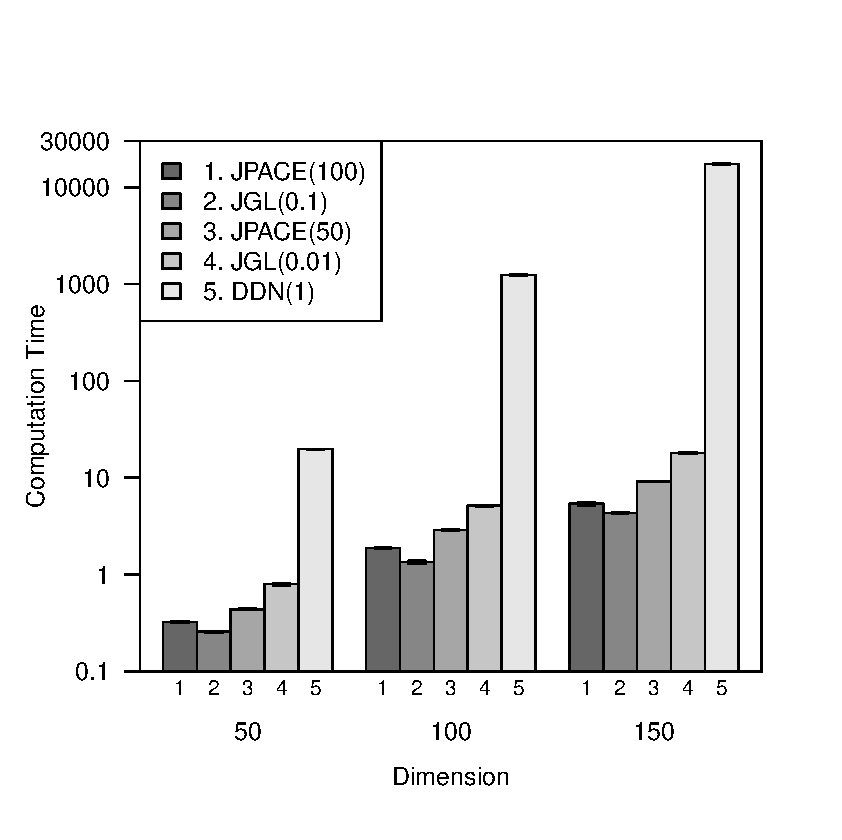
\epsfig{file=fig/time_den_a.eps,width=0.9\textwidth,height=0.35\textheight}}
  \centerline{(c) Dense, Structure}
\end{minipage}
\begin{minipage}[b]{.48\linewidth}
  \centering   \centerline{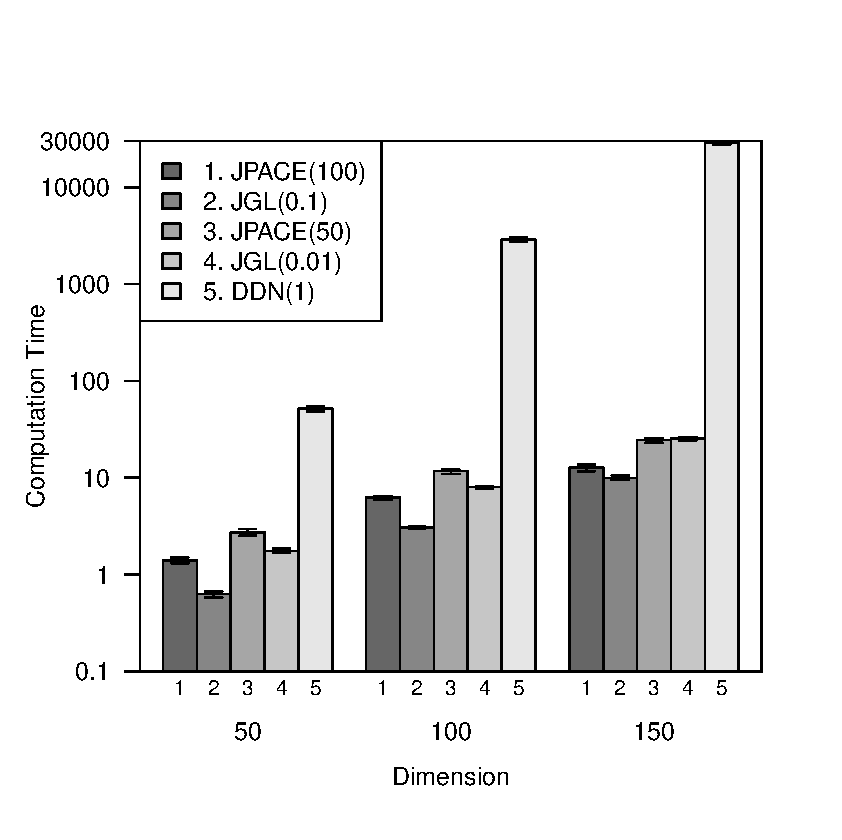
\epsfig{file=fig/time_den_b.eps,width=0.9\textwidth,height=0.35\textheight}}
  \centerline{(d) Dense, Direction}
\end{minipage}
\caption{Comparison of computing times. In each panel, columns represent JPACE$(50,50)$, JPACE$(100,50)$, JGL($0.01,0.15$), JGL($0.1,0.15$), DDN(1),
respectively. The numbers in parenthesis are tuning parameters 
$(\lambda_1, \lambda_2)$ for JPACE and JGL and $\lambda$ for DDN. 
The tuning parameters were chosen for the number of estimated 
differential edges to be similar.}
\end{center}
\end{figure}



\begin{figure}[htb!]
 \begin{minipage}[c]{.45\linewidth}
  \centering
\centerline{\epsfig{file=fig/axial.eps,width=12cm,height=7cm}}
\end{minipage}
 \begin{minipage}[c]{.45\linewidth}
  \centering
\centerline{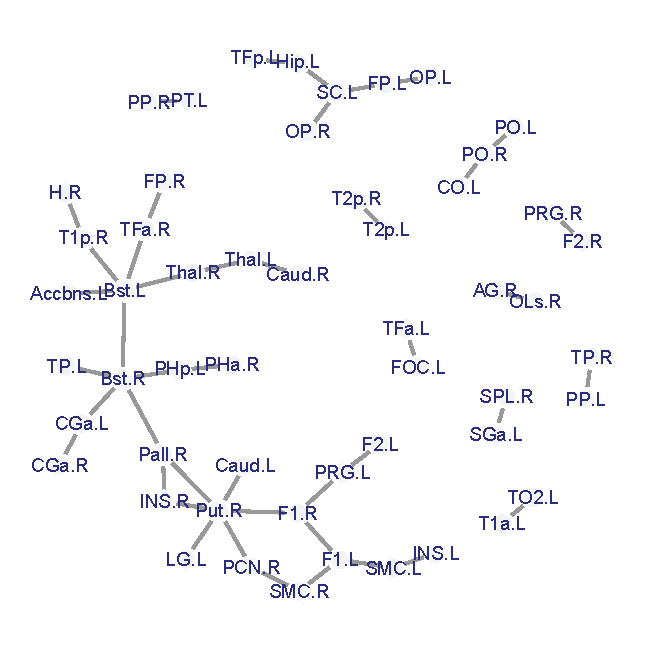
\epsfig{file=fig/Diff_net.eps,width=0.8\textwidth,height=6cm}}
\end{minipage}
  \caption{Differential network between AD and HC in Axial view}
\label{axial}
\end{figure}


\clearpage




\begin{table}[htb!]
\caption{Area under curve (AUC) of ROC curves.
To obtain the ROC curves, JPACE and JGL were conducted for various $\lambda_2$ with the fixed $\lambda_1^*$ chosen by the AIC.}
\medskip
\centering
{\footnotesize
\begin{tabular}{|c|c|c|c|c|c|} \cline{1-6}
\multirow{2}{*}{Network}	&	\multirow{2}{*}{Difference type}	&	\multirow{2}{*}{Method}	&	\multicolumn{3}{|c|}{$p$}					\\	\cline{4-6}
	&		&		&	50	&	100	&	150	\\	\hline
\multirow{8}{*}{Sparse}	&	\multirow{4}{*}{Structure}	&	JPACE($\lambda_1^*$)	&	98.18	&	99.41	&	98.65	\\	
	&		&	JGL($\lambda_1^*$)	&	95.71	&	97.23	&	92.99	\\	
	&		&	JGL($\lambda_1=0$)	&	96.64	&	98.43	&	95.72	\\	
	&		&	DDN	&	94.54	&	96.23	&	91.29	\\	\cline{2-6}
	&	\multirow{4}{*}{Direction}	&	JPACE($\lambda_1*$)	&	99.99	&	99.99	&	99.97	\\	
	&		&	JGL($\lambda_1^*$)	&	99.83	&	99.90	&	99.01	\\	
	&		&	JGL($\lambda_1=0$)	&	99.99	&	99.81	&	99.99	\\	
	&		&	DDN	&	98.29	&	96.46	&	93.92	\\	\hline
\multirow{8}{*}{Dense}	&	\multirow{4}{*}{Structure}	&	JPACE($\lambda_1^*$)	&	98.44	&	99.15	&	99.42	\\	
	&		&	JGL($\lambda_1^*$)	&	67.89	&	62.20	&	56.59	\\	
	&		&	JGL($\lambda_1=0$)	&	96.97	&	97.60	&	97.48	\\	
	&		&	DDN	&	95.69	&	96.91	&	95.86	\\	\cline{2-6}
	&	\multirow{4}{*}{Direction}	&	JPACE($\lambda_1^*$)	&	99.99	&	99.99	&	99.99	\\	
	&		&	JGL($\lambda_1^*$)	&	99.10	&	99.78	&	99.95	\\	
	&		&	JGL($\lambda_1=0$)	&	99.97	&	99.99	&	99.99	\\	
	&		&	DDN	&	93.75	&	95.69	&	96.27	\\	\hline

\end{tabular}
}
\end{table}


\begin{table}[htb!]
\caption{{\bf (C1)} Results for structural differences between two sparse
networks: the values are average over 50 replicates.
Standard errors are in parentheses.
}
\medskip
\centering
{ %\scriptsize
\begin{tabular}{||c|c|c||c|c|c|c|c|c|c||c} \cline{1-10}
$p$  &  $|E_d|$  & Method & $|\hat{E}_d|$ & TP & FP & SPE & SEN & FDR & MCC \\ \hline 
\multirow{12}{*}{50}  &\multirow{6}{*}{15}  & \multirow{2}{*}{JPACE} &20.48 & 10.20 & 10.28 & 99.59 & 68.00 & 42.36 & 60.48 \\ 
& & & (1.37) & (0.32) & (1.17) & (0.05) & (2.15) & (2.70) & (1.28) \\ \cline{3-10} 
& & \multirow{2}{*}{JGL} & 28.14 & 12.32 & 15.82 & 98.69 & 82.13 & 53.47 & 60.56 \\ 
 & & & (1.19) & (0.25) & (1.07) & (0.09) & (1.65) & (1.61) & (1.20) \\ \cline{3-10} 
& & \multirow{2}{*}{DDN} & 10.28 & 7.28 & 3.00 & 99.75 & 48.53 & 27.29 & 58.40 \\ 
 & & & (0.41) & (0.29) & (0.30) & (0.02) & (1.91) & (2.13) & (1.67) \\\cline{2-10} 
  &\multirow{6}{*}{30}  & \multirow{2}{*}{JPACE} &39.92 & 22.10 & 17.82 & 99.28 & 73.67 & 41.00 & 64.79 \\ 
& & & (1.73) & (0.33) & (1.54) & (0.06) & (1.09) & (1.84) & (0.98) \\ \cline{3-10} 
& & \multirow{2}{*}{JGL} & 82.06 & 26.88 & 55.18 & 95.38 & 89.60 & 65.40 & 53.56 \\ 
 & & & (2.76) & (0.27) & (2.58) & (0.22) & (0.92) & (1.17) & (0.78) \\ \cline{3-10} 
& & \multirow{2}{*}{DDN} & 11.90 & 10.24 & 1.66 & 99.86 & 34.13 & 11.05 & 52.77 \\ 
 & & & (0.78) & (0.61) & (0.24) & (0.02) & (2.02) & (1.39) & (1.60) \\\cline{1-10} 
\multirow{12}{*}{100}  &\multirow{6}{*}{15}  & \multirow{2}{*}{JPACE} &15.48 & 9.80 & 5.68 & 99.94 & 65.33 & 32.73 & 65.09 \\ 
& & & (0.88) & (0.33) & (0.61) & (0.01) & (2.17) & (1.65) & (0.96) \\ \cline{3-10} 
& & \multirow{2}{*}{JGL} & 31.82 & 11.44 & 20.38 & 99.59 & 76.27 & 62.50 & 52.95 \\ 
 & & & (1.15) & (0.20) & (1.08) & (0.02) & (1.34) & (1.08) & (0.96) \\ \cline{3-10} 
& & \multirow{2}{*}{DDN} & 10.18 & 5.14 & 5.04 & 99.90 & 34.27 & 41.51 & 42.59 \\ 
 & & & (0.68) & (0.30) & (0.52) & (0.01) & (1.99) & (3.41) & (1.77) \\\cline{2-10} 
  &\multirow{6}{*}{30}  & \multirow{2}{*}{JPACE} &28.80 & 19.00 & 9.80 & 99.90 & 63.33 & 32.15 & 65.00 \\ 
& & & (0.99) & (0.40) & (0.72) & (0.01) & (1.34) & (1.43) & (0.87) \\ \cline{3-10} 
& & \multirow{2}{*}{JGL} & 52.98 & 22.54 & 30.44 & 99.38 & 75.13 & 54.81 & 57.32 \\ 
 & & & (2.12) & (0.37) & (1.90) & (0.04) & (1.25) & (1.50) & (0.89) \\ \cline{3-10} 
& & \multirow{2}{*}{DDN} & 9.20 & 6.46 & 2.74 & 99.94 & 21.53 & 25.87 & 38.55 \\ 
 & & & (0.65) & (0.38) & (0.38) & (0.01) & (1.27) & (2.97) & (1.46) \\\cline{1-10} 
\multirow{12}{*}{150}  &\multirow{6}{*}{15}  & \multirow{2}{*}{JPACE} &8.88 & 5.10 & 3.78 & 99.98 & 34.00 & 39.14 & 43.88 \\ 
& & & (0.64) & (0.33) & (0.40) & (0.00) & (2.18) & (2.42) & (1.78) \\ \cline{3-10} 
& & \multirow{2}{*}{JGL} & 37.60 & 9.56 & 28.04 & 99.75 & 63.73 & 73.70 & 40.56 \\ 
 & & & (1.32) & (0.27) & (1.24) & (0.01) & (1.80) & (0.87) & (1.08) \\ \cline{3-10} 
& & \multirow{2}{*}{DDN} & 6.22 & 0.96 & 5.26 & 99.95 & 6.40 & 52.51 & 15.88 \\ 
 & & & (2.10) & (0.03) & (2.10) & (0.02) & (0.19) & (5.58) & (1.14) \\\cline{2-10} 
  &\multirow{6}{*}{30}  & \multirow{2}{*}{JPACE} &22.44 & 13.40 & 9.04 & 99.96 & 44.67 & 37.50 & 51.53 \\ 
& & & (1.33) & (0.65) & (0.80) & (0.00) & (2.15) & (1.63) & (1.37) \\ \cline{3-10} 
& & \multirow{2}{*}{JGL} & 60.74 & 20.38 & 40.36 & 99.64 & 67.93 & 65.52 & 47.95 \\ 
 & & & (1.86) & (0.35) & (1.66) & (0.01) & (1.18) & (0.80) & (0.70) \\ \cline{3-10} 
& & \multirow{2}{*}{DDN} & 6.67 & 1.02 & 5.65 & 99.95 & 3.40 & 43.13 & 12.35 \\ 
 & & & (1.74) & (0.06) & (1.72) & (0.02) & (0.21) & (6.13) & (0.94) \\\cline{1-10} 

\end{tabular}
}
\end{table}



\begin{table}[htb!]
\caption{{\bf (C2)} Results for directional differences between two sparse
networks: the values are average over 50 replicates.
Standard errors are in parentheses.}
\medskip
\centering
{ %\scriptsize
\begin{tabular}{||c|c|c||c|c|c|c|c|c|c||c} \cline{1-10}
$p$  &  $|E_d|$  & Method & $|\hat{E}_d|$ & TP & FP & SPE & SEN & FDR & MCC \\ \hline 
\multirow{12}{*}{50}  &\multirow{6}{*}{15}  & \multirow{2}{*}{JPACE} &52.04 & 15.00 & 37.04 & 98.51 & 100.00 & 69.65 & 54.36 \\ 
& & & (1.77) & (0.00) & (1.77) & (0.07) & (0.00) & (0.96) & (0.89) \\ \cline{3-10} 
& & \multirow{2}{*}{JGL} & 75.68 & 14.82 & 60.86 & 94.97 & 98.80 & 79.31 & 43.76 \\ 
 & & & (2.67) & (0.05) & (2.66) & (0.22) & (0.37) & (0.68) & (0.76) \\ \cline{3-10} 
& & \multirow{2}{*}{DDN} & 44.56 & 11.72 & 32.84 & 97.29 & 78.13 & 72.99 & 44.13 \\ 
 & & & (2.26) & (0.58) & (1.84) & (0.15) & (3.88) & (1.08) & (1.76) \\\cline{2-10} 
  &\multirow{6}{*}{30}  & \multirow{2}{*}{JPACE} &82.34 & 30.00 & 52.34 & 97.88 & 100.00 & 62.30 & 60.50 \\ 
& & & (2.19) & (0.00) & (2.19) & (0.09) & (0.00) & (1.00) & (0.82) \\ \cline{3-10} 
& & \multirow{2}{*}{JGL} & 94.70 & 29.90 & 64.80 & 94.58 & 99.67 & 66.62 & 55.73 \\ 
 & & & (3.12) & (0.05) & (3.11) & (0.26) & (0.17) & (1.17) & (1.01) \\ \cline{3-10} 
& & \multirow{2}{*}{DDN} & 39.82 & 23.54 & 16.28 & 98.64 & 78.47 & 35.95 & 67.16 \\ 
 & & & (2.71) & (1.30) & (1.65) & (0.14) & (4.32) & (2.07) & (2.18) \\\cline{1-10} 
\multirow{12}{*}{100}  &\multirow{6}{*}{15}  & \multirow{2}{*}{JPACE} &41.50 & 15.00 & 26.50 & 99.73 & 100.00 & 62.42 & 60.93 \\ 
& & & (1.20) & (0.00) & (1.20) & (0.01) & (0.00) & (1.06) & (0.86) \\ \cline{3-10} 
& & \multirow{2}{*}{JGL} & 39.34 & 13.94 & 25.40 & 99.49 & 92.93 & 62.55 & 58.40 \\ 
 & & & (1.52) & (0.13) & (1.48) & (0.03) & (0.86) & (1.18) & (0.96) \\ \cline{3-10} 
& & \multirow{2}{*}{DDN} & 14.02 & 2.70 & 11.32 & 99.77 & 18.00 & 45.87 & 23.53 \\ 
 & & & (2.06) & (0.27) & (1.84) & (0.04) & (1.78) & (5.76) & (0.90) \\\cline{2-10} 
  &\multirow{6}{*}{30}  & \multirow{2}{*}{JPACE} &80.68 & 29.96 & 50.72 & 99.49 & 99.87 & 61.93 & 61.31 \\ 
& & & (1.80) & (0.03) & (1.79) & (0.02) & (0.09) & (0.87) & (0.69) \\ \cline{3-10} 
& & \multirow{2}{*}{JGL} & 74.76 & 28.18 & 46.58 & 99.05 & 93.93 & 60.75 & 60.05 \\ 
 & & & (2.32) & (0.19) & (2.22) & (0.05) & (0.64) & (1.06) & (0.76) \\ \cline{3-10} 
& & \multirow{2}{*}{DDN} & 11.22 & 3.86 & 7.36 & 99.85 & 12.87 & 54.04 & 21.57 \\ 
 & & & (1.00) & (0.29) & (0.80) & (0.02) & (0.96) & (3.57) & (0.91) \\\cline{1-10} 
\multirow{12}{*}{150}  &\multirow{6}{*}{15}  & \multirow{2}{*}{JPACE} &38.78 & 14.94 & 23.84 & 99.89 & 99.60 & 60.45 & 62.54 \\ 
& & & (0.98) & (0.03) & (0.97) & (0.00) & (0.23) & (0.85) & (0.70) \\ \cline{3-10} 
& & \multirow{2}{*}{JGL} & 43.06 & 12.18 & 30.88 & 99.72 & 81.20 & 70.63 & 48.40 \\ 
 & & & (1.40) & (0.24) & (1.31) & (0.01) & (1.59) & (0.85) & (0.89) \\ \cline{3-10} 
& & \multirow{2}{*}{DDN} & 9.70 & 0.98 & 8.72 & 99.92 & 6.53 & 71.10 & 12.23 \\ 
 & & & (2.28) & (0.02) & (2.28) & (0.02) & (0.13) & (4.05) & (0.92) \\\cline{2-10} 
  &\multirow{6}{*}{30}  & \multirow{2}{*}{JPACE} &78.70 & 29.98 & 48.72 & 99.78 & 99.93 & 61.24 & 62.03 \\ 
& & & (1.48) & (0.02) & (1.48) & (0.01) & (0.07) & (0.74) & (0.59) \\ \cline{3-10} 
& & \multirow{2}{*}{JGL} & 76.16 & 26.02 & 50.14 & 99.55 & 86.73 & 64.50 & 55.01 \\ 
 & & & (2.38) & (0.26) & (2.28) & (0.02) & (0.86) & (0.94) & (0.75) \\ \cline{3-10} 
& & \multirow{2}{*}{DDN} & 1.02 & 1.02 & 0.00 & 100.00 & 3.40 & 0.00 & 18.38 \\ 
 & & & (0.02) & (0.02) & (0.00) & (0.00) & (0.07) & (0.00) & (0.15) \\\cline{1-10} 
\end{tabular}
}
\end{table}




\begin{table}[htb!]
\caption{{\bf (C3)} Results for structural differences between two dense
networks: the values are average over 50 replicates.
Standard errors are in parentheses.}
\medskip
\centering
{ %\scriptsize
\begin{tabular}{||c|c|c||c|c|c|c|c|c|c||c} \cline{1-10}
$p$  &  $|E_d|$  & Method & $|\hat{E}_d|$ & TP & FP & SPE & SEN & FDR & MCC \\ \hline 
\multirow{12}{*}{50}  &\multirow{6}{*}{15}  & \multirow{2}{*}{JPACE} &10.36 & 7.32 & 3.04 & 99.88 & 48.80 & 20.85 & 57.84 \\ 
& & & (0.91) & (0.51) & (0.48) & (0.02) & (3.38) & (2.40) & (2.23) \\ \cline{3-10} 
& & \multirow{2}{*}{JGL} & 6.72 & 3.30 & 3.42 & 99.72 & 22.00 & 50.24 & 28.84 \\ 
 & & & (0.73) & (0.37) & (0.48) & (0.04) & (2.45) & (4.07) & (2.76) \\ \cline{3-10} 
& & \multirow{2}{*}{DDN} & 7.58 & 6.20 & 1.38 & 99.89 & 41.33 & 15.78 & 57.12 \\ 
 & & & (0.46) & (0.33) & (0.21) & (0.02) & (2.19) & (1.96) & (1.86) \\\cline{2-10} 
  &\multirow{6}{*}{30}  & \multirow{2}{*}{JPACE} &24.50 & 16.36 & 8.14 & 99.67 & 54.53 & 22.76 & 60.82 \\ 
& & & (2.15) & (0.99) & (1.27) & (0.05) & (3.28) & (2.56) & (1.50) \\ \cline{3-10} 
& & \multirow{2}{*}{JGL} & 5.80 & 4.10 & 1.70 & 99.86 & 13.67 & 20.70 & 23.40 \\ 
 & & & (0.97) & (0.67) & (0.36) & (0.03) & (2.24) & (4.14) & (3.02) \\ \cline{3-10} 
& & \multirow{2}{*}{DDN} & 7.64 & 7.26 & 0.38 & 99.97 & 24.20 & 3.77 & 46.19 \\ 
 & & & (0.49) & (0.45) & (0.11) & (0.01) & (1.50) & (0.99) & (1.66) \\\cline{1-10} 
\multirow{12}{*}{100}  &\multirow{6}{*}{15}  & \multirow{2}{*}{JPACE} &2.90 & 2.68 & 0.22 & 100.00 & 17.87 & 2.43 & 38.28 \\ 
& & & (0.40) & (0.33) & (0.09) & (0.00) & (2.18) & (0.91) & (2.03) \\ \cline{3-10} 
& & \multirow{2}{*}{JGL} & 2.82 & 0.50 & 2.32 & 99.95 & 3.33 & 69.17 & 5.77 \\ 
 & & & (0.51) & (0.13) & (0.41) & (0.01) & (0.86) & (5.90) & (1.41) \\ \cline{3-10} 
& & \multirow{2}{*}{DDN} & 6.44 & 5.26 & 1.18 & 99.98 & 35.07 & 15.02 & 53.06 \\ 
 & & & (0.40) & (0.30) & (0.20) & (0.00) & (1.97) & (2.30) & (1.73) \\\cline{2-10} 
  &\multirow{6}{*}{30}  & \multirow{2}{*}{JPACE} &5.48 & 5.10 & 0.38 & 100.00 & 17.00 & 2.75 & 36.38 \\ 
& & & (0.77) & (0.65) & (0.16) & (0.00) & (2.17) & (0.89) & (2.35) \\ \cline{3-10} 
& & \multirow{2}{*}{JGL} & 2.88 & 0.80 & 2.08 & 99.96 & 2.67 & 65.78 & 5.88 \\ 
 & & & (0.51) & (0.19) & (0.35) & (0.01) & (0.62) & (5.62) & (1.22) \\ \cline{3-10} 
& & \multirow{2}{*}{DDN} & 7.78 & 7.16 & 0.62 & 99.99 & 23.87 & 5.76 & 46.10 \\ 
 & & & (0.47) & (0.39) & (0.14) & (0.00) & (1.30) & (1.29) & (1.31) \\\cline{1-10} 
\multirow{12}{*}{150}  &\multirow{6}{*}{15}  & \multirow{2}{*}{JPACE} &2.74 & 2.60 & 0.14 & 100.00 & 17.33 & 1.67 & 37.83 \\ 
& & & (0.39) & (0.34) & (0.07) & (0.00) & (2.29) & (0.75) & (2.15) \\ \cline{3-10} 
& & \multirow{2}{*}{JGL} & 2.98 & 0.44 & 2.54 & 99.98 & 2.93 & 72.47 & 5.16 \\ 
 & & & (0.48) & (0.12) & (0.39) & (0.00) & (0.79) & (5.53) & (1.21) \\ \cline{3-10} 
& & \multirow{2}{*}{DDN} & 6.32 & 4.72 & 1.60 & 99.99 & 31.47 & 20.19 & 48.33 \\ 
 & & & (0.43) & (0.29) & (0.22) & (0.00) & (1.91) & (2.50) & (1.59) \\\cline{2-10} 
  &\multirow{6}{*}{30}  & \multirow{2}{*}{JPACE} &4.94 & 4.86 & 0.08 & 100.00 & 16.20 & 0.84 & 38.25 \\ 
& & & (0.43) & (0.42) & (0.05) & (0.00) & (1.39) & (0.48) & (1.64) \\ \cline{3-10} 
& & \multirow{2}{*}{JGL} & 2.48 & 0.48 & 2.00 & 99.98 & 1.60 & 59.94 & 5.04 \\ 
 & & & (0.45) & (0.13) & (0.36) & (0.00) & (0.44) & (6.34) & (1.12) \\ \cline{3-10} 
& & \multirow{2}{*}{DDN} & 1.02 & 1.02 & 0.00 & 100.00 & 3.40 & 0.00 & 18.39 \\ 
 & & & (0.02) & (0.02) & (0.00) & (0.00) & (0.07) & (0.00) & (0.15) \\\cline{1-10} 
\end{tabular}
}
\end{table}



\begin{table}[htb!]
\caption{{\bf (C4)} Results for directional differences between two dense
networks: the values are average over 50 replicates.
Standard errors are in parentheses.}
\medskip
\centering
{ %\scriptsize
\begin{tabular}{||c|c|c||c|c|c|c|c|c|c||c} \cline{1-10}
$p$  &  $|E_d|$  & Method & $|\hat{E}_d|$ & TP & FP & SPE & SEN & FDR & MCC \\ \hline 
\multirow{12}{*}{50}  &\multirow{6}{*}{15}  & \multirow{2}{*}{JPACE} &36.84 & 15.00 & 21.84 & 99.12 & 100.00 & 58.14 & 64.19 \\ 
& & & (0.87) & (0.00) & (0.87) & (0.03) & (0.00) & (1.01) & (0.78) \\ \cline{3-10} 
& & \multirow{2}{*}{JGL} & 62.14 & 14.72 & 47.42 & 96.08 & 98.13 & 73.98 & 48.90 \\ 
 & & & (2.55) & (0.08) & (2.53) & (0.21) & (0.51) & (1.23) & (1.13) \\ \cline{3-10} 
& & \multirow{2}{*}{DDN} & 20.14 & 14.66 & 5.48 & 99.55 & 97.73 & 24.13 & 85.41 \\ 
 & & & (0.69) & (0.14) & (0.64) & (0.05) & (0.91) & (1.93) & (1.12) \\\cline{2-10} 
  &\multirow{6}{*}{30}  & \multirow{2}{*}{JPACE} &95.22 & 30.00 & 65.22 & 97.36 & 100.00 & 66.81 & 56.50 \\ 
& & & (3.07) & (0.00) & (3.07) & (0.12) & (0.00) & (1.11) & (0.97) \\ \cline{3-10} 
& & \multirow{2}{*}{JGL} & 321.96 & 29.96 & 292.00 & 75.56 & 99.87 & 90.64 & 26.56 \\ 
 & & & (3.60) & (0.03) & (3.60) & (0.30) & (0.09) & (0.10) & (0.20) \\ \cline{3-10} 
& & \multirow{2}{*}{DDN} & 4.30 & 2.18 & 2.12 & 99.82 & 7.27 & 15.90 & 20.24 \\ 
 & & & (0.81) & (0.31) & (0.57) & (0.05) & (1.04) & (3.83) & (0.90) \\\cline{1-10} 
\multirow{12}{*}{100}  &\multirow{6}{*}{15}  & \multirow{2}{*}{JPACE} &27.98 & 15.00 & 12.98 & 99.87 & 100.00 & 43.40 & 74.69 \\ 
& & & (0.95) & (0.00) & (0.95) & (0.01) & (0.00) & (1.84) & (1.23) \\ \cline{3-10} 
& & \multirow{2}{*}{JGL} & 61.24 & 14.94 & 46.30 & 99.06 & 99.60 & 72.31 & 51.50 \\ 
 & & & (3.29) & (0.03) & (3.29) & (0.07) & (0.23) & (1.38) & (1.30) \\ \cline{3-10} 
& & \multirow{2}{*}{DDN} & 35.54 & 1.17 & 34.37 & 99.30 & 7.83 & 12.83 & 23.06 \\ 
 & & & (20.51) & (0.09) & (20.42) & (0.41) & (0.63) & (4.94) & (1.18) \\\cline{2-10} 
  &\multirow{6}{*}{30}  & \multirow{2}{*}{JPACE} &66.14 & 30.00 & 36.14 & 99.64 & 100.00 & 53.49 & 67.87 \\ 
& & & (1.53) & (0.00) & (1.53) & (0.02) & (0.00) & (1.04) & (0.77) \\ \cline{3-10} 
& & \multirow{2}{*}{JGL} & 558.80 & 30.00 & 528.80 & 89.25 & 100.00 & 94.60 & 21.94 \\ 
 & & & (6.19) & (0.00) & (6.19) & (0.13) & (0.00) & (0.06) & (0.14) \\ \cline{3-10} 
& & \multirow{2}{*}{DDN} & 1.02 & 1.02 & 0.00 & 100.00 & 3.40 & 0.00 & 18.35 \\ 
 & & & (0.02) & (0.02) & (0.00) & (0.00) & (0.07) & (0.00) & (0.15) \\\cline{1-10} 
\multirow{12}{*}{150}  &\multirow{6}{*}{15}  & \multirow{2}{*}{JPACE} &28.26 & 15.00 & 13.26 & 99.94 & 100.00 & 45.27 & 73.69 \\ 
& & & (0.74) & (0.00) & (0.74) & (0.00) & (0.00) & (1.31) & (0.90) \\ \cline{3-10} 
& & \multirow{2}{*}{JGL} & 65.56 & 14.98 & 50.58 & 99.55 & 99.87 & 75.42 & 49.01 \\ 
 & & & (2.67) & (0.02) & (2.67) & (0.02) & (0.13) & (0.92) & (0.93) \\ \cline{3-10} 
& & \multirow{2}{*}{DDN} & 7.94 & 3.70 & 4.24 & 99.96 & 24.67 & 31.00 & 34.96 \\ 
 & & & (0.95) & (0.40) & (0.68) & (0.01) & (2.66) & (4.29) & (1.96) \\\cline{2-10} 
  &\multirow{6}{*}{30}  & \multirow{2}{*}{JPACE} &74.90 & 30.00 & 44.90 & 99.80 & 100.00 & 58.48 & 64.08 \\ 
& & & (2.04) & (0.00) & (2.04) & (0.01) & (0.00) & (1.13) & (0.87) \\ \cline{3-10} 
& & \multirow{2}{*}{JGL} & 483.82 & 30.00 & 453.82 & 95.93 & 100.00 & 93.74 & 24.48 \\ 
 & & & (6.59) & (0.00) & (6.59) & (0.06) & (0.00) & (0.09) & (0.18) \\ \cline{3-10} 
& & \multirow{2}{*}{DDN} & 16.64 & 1.08 & 15.56 & 99.86 & 3.60 & 60.04 & 9.71 \\ 
 & & & (4.07) & (0.04) & (4.04) & (0.04) & (0.13) & (5.90) & (0.89) \\\cline{1-10} 

\end{tabular}
}
\end{table}





\begin{table}[htb!]
\begin{center}
\scalebox{1}{
\begin{tabular}{|ll|}
\hline
%ROI 1		&	ROI 2		 \\\hline
L.Brain-Stem	&	R.Brain-Stem 	\\
L.Brain-Stem	&	R.Thalamus 	\\
R.Insular Cortex 	&	R.Putamen	\\
R.Insular Cortex 	&	R.Pallidum 	\\
L.Middle Temporal Gyrus, posterior division	&	R.Middle Temporal Gyrus, posterior division	\\
R.Pallidum 	&	R.Brain-Stem 	\\
L.Parahippocampal Gyrus, posterior division	&	R.Brain-Stem 	\\
L.Caudate	&	R.Putamen	\\
R.Putamen	&	R.Pallidum 	\\
L.Thalamus 	&	R.Caudate	\\
L.Superior Frontal Gyrus 	&	L.Juxtapositional Lobule Cortex	\\
L.Brain-Stem 	&	R.Superior Temporal Gyrus, posterior division	\\
L.Thalamus 	&	R.Thalamus 	\\
L.Parietal Operculum Cortex	&	R.Parietal Operculum Cortex	\\
L.Planum Polare	&	R.Temporal Pole	\\
L.Frontal Orbital Cortex	&	L.Temporal Fusiform Cortex, anterior division	\\
L.FRONTAL POLE	&	L.Subcallosal Cortex	\\
L.Supramarginal Gyrus, anterior division	&	R.Superior Parietal Lobule	\\
R.Superior Frontal Gyrus 	&	R.Putamen	\\
L.Parahippocampal Gyrus, posterior division	&	R.Parahippocampal Gyrus, anterior division	\\
R.Angular Gyrus	&	R.Lateral Occipital Cortex, superoir division	\\
L.Brain-Stem 	&	L.Accumbens 	\\
L.FRONTAL POLE	&	L.Occipital Pole	\\
L.Lingual Gyrus	&	R.Putamen	\\
R.Middle Frontal Gyrus 	&	R.Precentral Gyrus	\\
L.Superior Temporal Gyrus, anterior division	&	L.Middle Temporal Gyrus, temporooccipital part	\\
L.Planum Temporale	&	R.Planum Polare	\\
L.Precentral Gyrus	&	R.Superior Frontal Gyrus 	\\
R.Precuneous Cortex	&	R.Putamen	\\
L.Subcallosal Cortex	&	R.Occipital Pole	\\
L.Middle Frontal Gyrus 	&	L.Precentral Gyrus	\\
R.Juxtapositional Lobule Cortex	&	R.Precuneous Cortex	\\
L.Superior Frontal Gyrus 	&	R.Superior Frontal Gyrus 	\\
L.Cingulate Gyrus, anterior division	&	R.Cingulate Gyrus, anterior division	\\
L.Superior Frontal Gyrus 	&	R.Juxtapositional Lobule Cortex	\\
L.Central Opercular Cortex	&	R.Parietal Operculum Cortex	\\
L.Insular Cortex 	&	L.Juxtapositional Lobule Cortex	\\
L.Temporal Fusiform Cortex, posterior division	&	L.Hippocampus 	\\
L.Subcallosal Cortex	&	L.Hippocampus 	\\
L.Brain-Stem 	&	R.Temporal Fusiform Cortex, anterior division	\\
R.FRONTAL POLE	&	R.Temporal Fusiform Cortex, anterior division	\\
L.Temporal Pole	&	R.Brain-Stem 	\\
R.Superior Temporal Gyrus, posterior division	&	R.Heschl's Gyrus	\\
L.Cingulate Gyrus, anterior division	&	R.Brain-Stem 	\\
 \hline
\end{tabular}  }
\caption{List of 44 differential edges in decreasing order of absolute difference. L. and R. are acronyms of left and right, respectively.}
\end{center}
\end{table}



\end{document}







